\appendix{}
\label{sec:appendix}

\begin{figure*}[thb!]
  \centering
  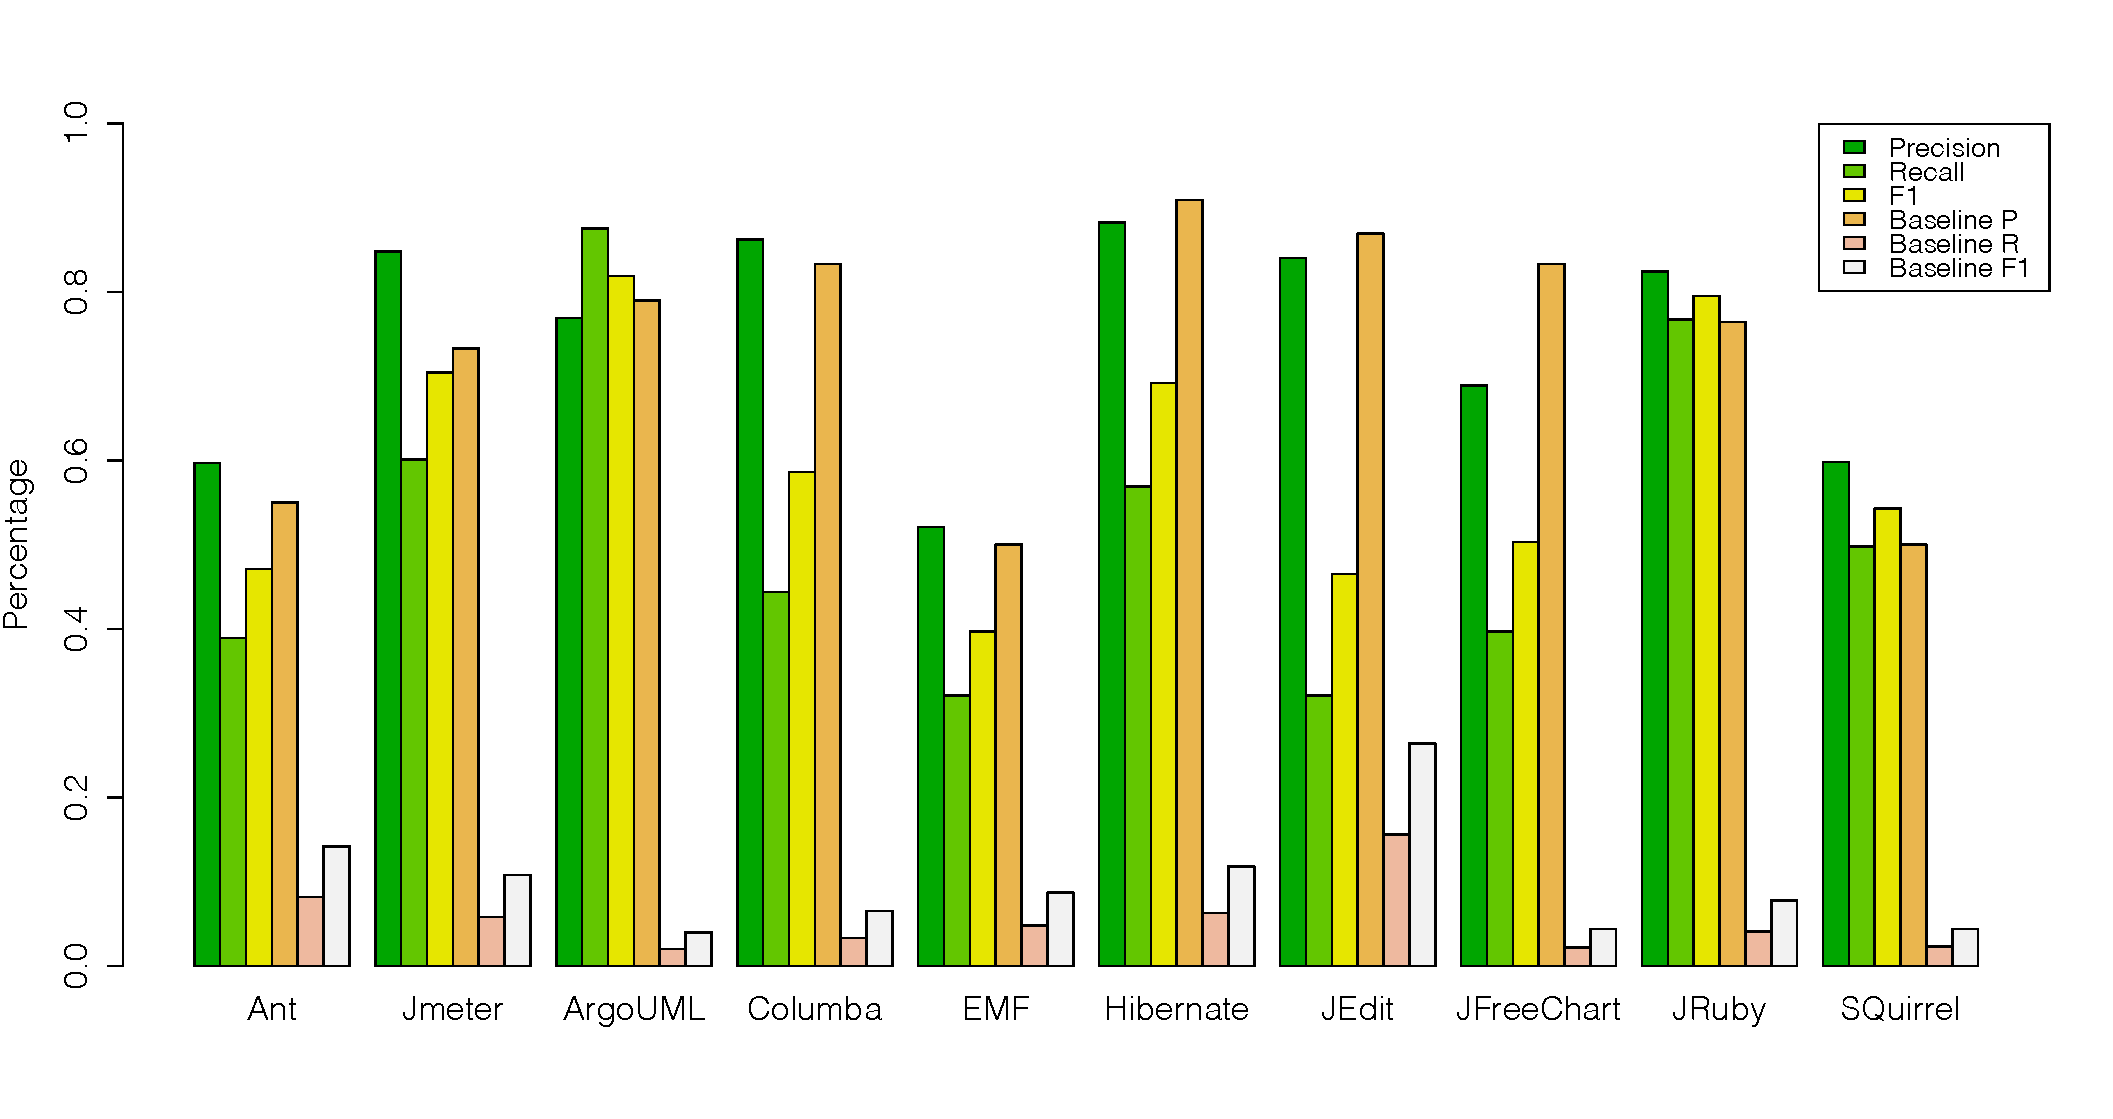
\includegraphics[width=0.90\textwidth]{figures/baseline_comparison_design.pdf}
  \caption{Classification design debt vs old approach}
  \label{fig:design_vs_baseline}
\end{figure*}

\begin{table*}[!hbt]
    \begin{center}
        \caption{Classification results vs Baseline vs Random for Design Debt}
        \label{tbl:classifier_results_vs_baseline_design}
        \begin{tabular}{l| c c c c c c c c c}
        \toprule
        \textbf{Project} & \textbf{P} & \textbf{R} & \textbf{F1} & \thead{Baseline\\P} & \thead{Baseline\\R} & \thead{Baseline\\F1} & \thead{Rdn\\P} & \thead{Rdn\\R} & \thead{Rdn\\F1} \\
        \midrule
        Apache Ant    &  0.554   &  0.484  &  0.517  & 0.55    & 0.082  & 0.142  &  0.023 &  0.5 &  0.045  \\
        Apache Jmeter &  0.808   &  0.668  &  0.731  & 0.733   & 0.058  & 0.108  &  0.04  &  0.5 &  0.075  \\
        ArgoUML       &  0.788   &  0.843  &  0.814  & 0.790   & 0.020  & 0.040  &  0.089 &  0.5 &  0.151  \\
        Columba       &  0.792   &  0.484  &  0.601  & 0.833   & 0.033  & 0.065  &  0.020 &  0.5 &  0.038  \\
        EMF           &  0.574   &  0.397  &  0.470  & 0.5     & 0.048  & 0.087  &  0.018 &  0.5 &  0.035  \\
        Hibernate     &  0.877   &  0.645  &  0.744  & 0.909   & 0.063  & 0.118  &  0.136 &  0.5 &  0.214  \\
        JEdit         &  0.779   &  0.378  &  0.509  & 0.869   & 0.156  & 0.264  &  0.019 &  0.5 &  0.037  \\
        JFreeChart    &  0.646   &  0.397  &  0.492  & 0.833   & 0.022  & 0.044  &  0.043 &  0.5 &  0.080  \\
        JRuby         &  0.798   &  0.770  &  0.783  & 0.764   & 0.041  & 0.078  &  0.075 &  0.5 &  0.131  \\
        SQuirrel      &  0.544   &  0.536  &  0.540  & 0.5     & 0.023  & 0.044  &  0.029 &  0.5 &  0.055  \\
        \bottomrule
        \end{tabular}
    \end{center}    
\end{table*}

\begin{table*}[!hbt]
    \begin{center}
        \caption{Classification results vs Baseline vs Random for Requirement Debt}
        \label{tbl:classifier_results_vs_baseline_requirement}
        \begin{tabular}{l| c c c c c c c c c}
        \toprule
        \textbf{Project} & \textbf{P} & \textbf{R} & \textbf{F1} & \thead{Baseline\\P} & \thead{Baseline\\R} & \thead{Baseline\\F1} & \thead{Rdn\\P} & \thead{Rdn\\R} & \thead{Rdn\\F1} \\
        \midrule
        Apache Ant    &  0.353 &  0.375 & 0.364 & 0.55  & 0.082 & 0.142  & 0.004 &0.5 & 0.008  \\
        Apache Jmeter &  0.167 &  0.545 & 0.255 & 0.733 & 0.058 & 0.108  & 0.003 &0.5 & 0.005  \\
        ArgoUML       &  0.802 &  0.722 & 0.760 & 0.790 & 0.020 & 0.040  & 0.071 &0.5 & 0.125  \\
        Columba       &  0.914 &  0.955 & 0.934 & 0.833 & 0.033 & 0.065  & 0.021 &0.5 &  0.04  \\
        EMF           &  0.800 &  0.250 & 0.381 & 0.5   & 0.048 & 0.087  & 0.004 &0.5 & 0.007  \\
        Hibernate     &  0.610 &  0.391 & 0.476 & 0.909 & 0.063 & 0.118  & 0.022 &0.5 & 0.042  \\
        JEdit         &  0.125 &  0.071 & 0.091 & 0.869 & 0.156 & 0.264  & 0.001 &0.5 & 0.003  \\
        JFreeChart    &  0.373 &  0.760 & 0.500 & 0.833 & 0.022 & 0.044  & 0.006 &0.5 & 0.011  \\
        JRuby         &  0.709 &  0.342 & 0.462 & 0.764 & 0.041 & 0.078  & 0.024 &0.5 & 0.045  \\
        SQuirrel      &  0.913 &  0.840 & 0.875 & 0.5   & 0.023 & 0.044  & 0.021 &0.5 &  0.04  \\
        \bottomrule
        \end{tabular}
    \end{center}    
\end{table*}

\clearpage

\begin{table}
    \begin{center}
        \caption{Technical Debt distribution per type}
        \label{tbl:td_distribution}
        \begin{tabular}{l|SSSSSSS}
        \toprule
        \multirow{2}{*}{Project} & \multicolumn{4}{c}{TD Distribution} \\ & {Design} & {Req.} & {Defect} & {Other} & \multirow{-2}{*}{Total TD comments} & \multirow{-2}{*}{Total comments} &  \multirow{-2}{*}{TD \%} \\
        \midrule
        Ant             & 95  & 16 & 13 & 10  & 134   & 4,140  & 3.2       \\
        Jmeter          & 316 & 22 & 22 & 15  & 375   & 8,163  & 4.6       \\
        ArgoUML         & 801 & 651& 127& 74  & 1653  & 9,788  & 16.8      \\
        Columba         & 126 & 134& 13 & 22  & 295   & 6,569  & 4.4       \\
        EMF             & 78  & 16 & 8  & 2   & 104   & 4,401  & 2.3       \\
        Hibernate       & 355 & 64 & 52 & 1   & 472   & 2,968  & 15.9      \\
        JEdit           & 196 & 14 & 43 & 3   & 256   & 10,322 & 2.4       \\
        JFreeChart      & 184 & 25 & 9  & 1   & 219   & 4,436  & 4.9       \\
        JRuby           & 343 & 114& 161& 8   & 626   & 4,901  & 12.7      \\
        SQuirrel        & 209 & 150& 24 & 3   & 386   & 7,330  & 5.2       \\
        \bottomrule
        \end{tabular}
    \end{center}    
\end{table}

\clearpage

\begin{table*}[!thb]
    \begin{center}
        \caption{Comparison between different classifiers design debt}
        \label{tbl:improvement_f1measure}
        \begin{tabular}{l| c c c c c c c c c }
        \toprule
        \thead{Project} & \thead{Logistic\\Regression\\Precision} & \thead{Logistic\\Regression\\Recall} & \thead{Logistic\\Regression\\F1 measure} & \thead{Naive\\Bayes\\Precision} & \thead{Naive\\Bayes\\Recall} & \thead{Naive\\Bayes\\F1 measure} & \thead{Binary\\Precision} & \thead{Binary\\Recall} & \thead{Binary\\F1 measure}\\
        \midrule                                                  
        Ant          &  0.554   &  0.484  &  0.517 &   0.072 &  0.874 &   0.134 &  0.620 &    0.516 & 0.563  \\
        ArgoUML      &  0.808   &  0.668  &  0.731 &   0.358 &  0.985 &   0.525 &  0.790 &    0.858 & 0.822  \\
        Columba      &  0.788   &  0.843  &  0.814 &   0.181 &  0.786 &   0.294 &  0.840 &    0.500 & 0.627  \\
        EMF          &  0.792   &  0.484  &  0.601 &   0.057 &  0.872 &   0.106 &  0.633 &    0.397 & 0.488  \\
        Hibernate    &  0.574   &  0.397  &  0.470 &   0.288 &  0.890 &   0.435 &  0.895 &    0.670 & 0.767  \\
        JEdit        &  0.877   &  0.645  &  0.744 &   0.227 &  0.791 &   0.353 &  0.807 &    0.342 & 0.480  \\
        JFreeChart   &  0.779   &  0.378  &  0.509 &   0.224 &  0.801 &   0.350 &  0.658 &    0.397 & 0.495  \\
        Jmeter       &  0.646   &  0.397  &  0.492 &   0.140 &  0.560 &   0.224 &  0.819 &    0.671 & 0.737  \\
        JRuby        &  0.798   &  0.770  &  0.783 &   0.275 &  0.971 &   0.429 &  0.815 &    0.808 & 0.811  \\
        SQuirrel     &  0.544   &  0.536  &  0.540 &   0.133 &  0.947 &   0.233 &  0.567 &    0.550 & 0.558  \\
        \bottomrule
        \end{tabular}
    \end{center}    
\end{table*}

\begin{table*}[!thb]
    \begin{center}
        \caption{Comparison between different classifiers requirement debt}
        \label{tbl:improvement_f1measure}
        \begin{tabular}{l| c c c c c c c c c }
        \toprule
        \thead{Project} & \thead{Logistic\\Regression\\Precision} & \thead{Logistic\\Regression\\Recall} & \thead{Logistic\\Regression\\F1 measure} & \thead{Naive\\Bayes\\Precision} & \thead{Naive\\Bayes\\Recall} & \thead{Naive\\Bayes\\F1 measure} & \thead{Binary\\Precision} & \thead{Binary\\Recall} & \thead{Binary\\F1 measure}\\
        \midrule                                                  
        Ant          &  0.353 &  0.375 & 0.364 & 0.015 &  0.868 &  0.030 &  0.462 & 0.375 &  0.414   \\
        ArgoUML      &  0.167 &  0.545 & 0.255 & 0.207 &  0.877 &  0.335 &  0.792 & 0.731 &  0.760   \\
        Columba      &  0.802 &  0.722 & 0.760 & 0.105 &  0.978 &  0.189 &  0.914 & 0.955 &  0.934   \\
        EMF          &  0.914 &  0.955 & 0.934 & 0.010 &  1.000 &  0.020 &  0.800 & 0.250 &  0.381   \\
        Hibernate    &  0.800 &  0.250 & 0.381 & 0.051 &  0.844 &  0.097 &  0.641 & 0.391 &  0.485   \\
        JEdit        &  0.610 &  0.391 & 0.476 & 0.010 &  0.786 &  0.020 &  0.143 & 0.071 &  0.095   \\
        JFreeChart   &  0.125 &  0.071 & 0.091 & 0.020 &  0.840 &  0.039 &  0.347 & 0.680 &  0.459   \\
        Jmeter       &  0.373 &  0.760 & 0.500 & 0.015 &  0.955 &  0.029 &  0.194 & 0.545 &  0.286   \\
        JRuby        &  0.709 &  0.342 & 0.462 & 0.074 &  0.904 &  0.137 &  0.702 & 0.351 &  0.468   \\
        SQuirrel     &  0.913 &  0.840 & 0.875 & 0.064 &  0.967 &  0.121 &  0.806 & 0.833 &  0.820   \\
        \bottomrule
        \end{tabular}
    \end{center}    
\end{table*} 

\clearpage

\begin{table}[!hbt]
    \begin{center}
        \caption{Design Debt features per project}
        \label{tbl:design_features_per_project}
        \begin{tabular}{l| c c c }
        \toprule
        \textbf{Project} & \thead{Design TD\\features} & \thead{No TD\\Features} & \thead{Total\\Features} \\
        \midrule
        Apache Ant    &  6,559 & 35,517 & 42,052  \\
        Apache Jmeter &  6,414 & 35,110 & 41,500  \\
        ArgoUML       &  4,802 & 33,894 & 38,689  \\
        Columba       &  6,555 & 34,446 & 40,977  \\
        EMF           &  6,636 & 35,331 & 41,943  \\
        Hibernate     &  6,071 & 35,476 & 41,524  \\
        JEdit         &  6,269 & 33,950 & 40,196  \\
        JFreeChart    &  6,551 & 35,544 & 42,171  \\
        JRuby         &  5,991 & 34,716 & 40,686  \\
        SQuirrel      &  6,116 & 31,863 & 37,955  \\
        \bottomrule
        \end{tabular}
    \end{center}    
\end{table}

\begin{table}[!hbt]
    \begin{center}
        \caption{Requirement Debt features per project}
        \label{tbl:requirement_features_per_project}
        \begin{tabular}{l| c c c }
        \toprule
        \textbf{Project} & \thead{Requirement TD\\features} & \thead{No TD\\Features} & \thead{Total\\Features} \\
        \midrule
        Apache Ant    & 3,015  & 35,926 & 38,888  \\
        Apache Jmeter & 3,456  & 35,165 & 38,568  \\
        ArgoUML       & 2,785  & 33,693 & 36,467  \\
        Columba       & 2,181  & 35,821 & 37,948  \\
        EMF           & 2,852  & 36,025 & 38,823  \\
        Hibernate     & 2,691  & 36,155 & 38,794  \\
        JEdit         & 3,194  & 34,092 & 37,233  \\
        JFreeChart    & 2,470  & 36,630 & 39,046  \\
        JRuby         & 3,129  & 34,856 & 37,931  \\
        SQuirrel      & 3,118  & 32,327 & 35,128  \\
        \bottomrule
        \end{tabular}
    \end{center}    
\end{table}

\clearpage

\begin{figure}[thb!]
  \centering
  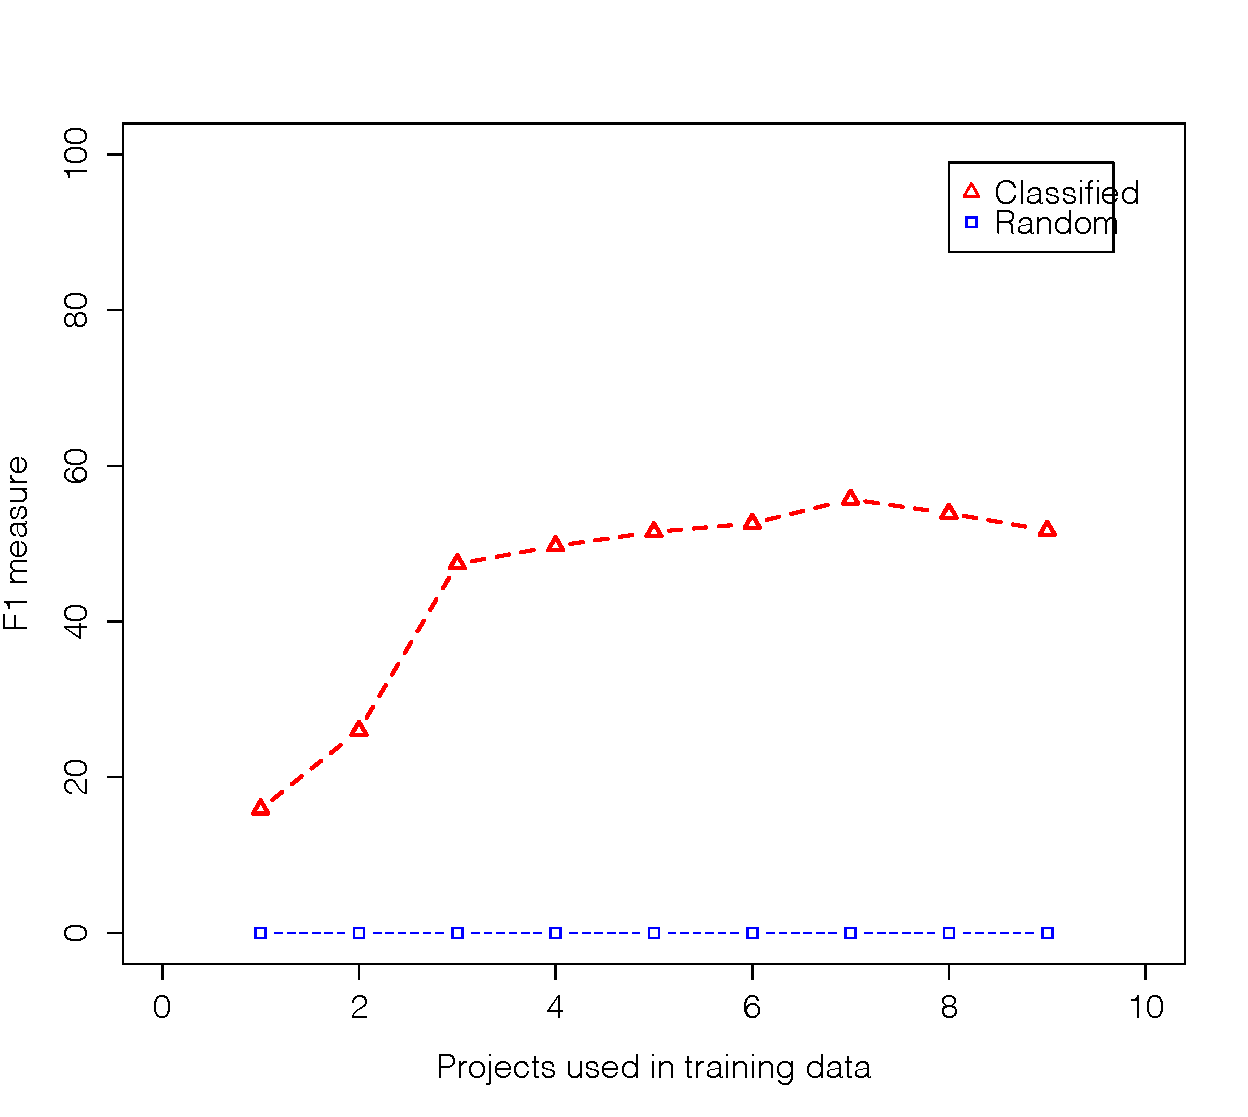
\includegraphics[width=0.50\textwidth]{figures/design_ant.pdf}
  \vspace{-3mm}
  \caption{Ant Design Debt classification}
  \label{fig:design_ant}
\end{figure}

\begin{figure}[thb!]
  \centering
  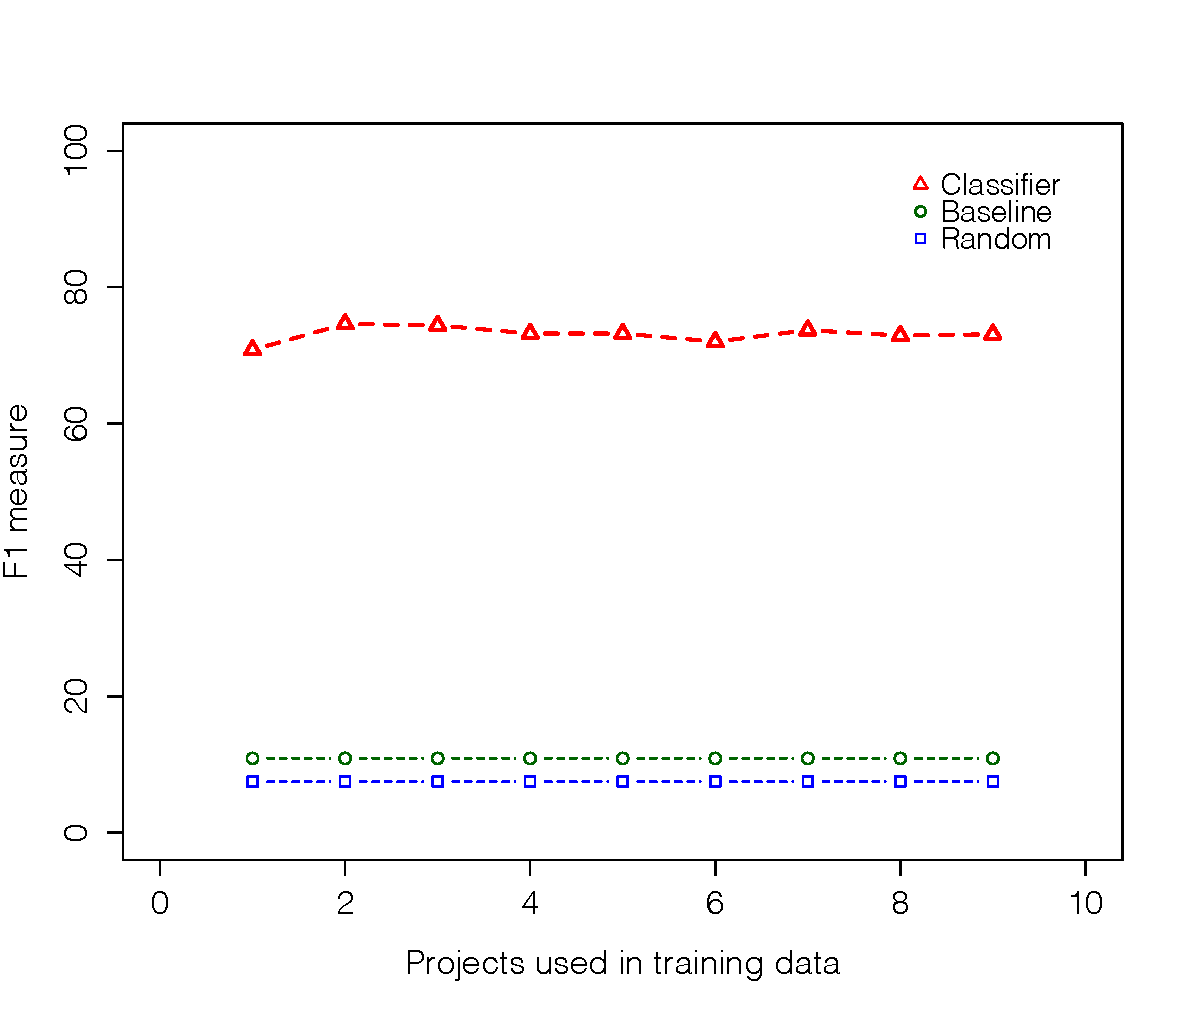
\includegraphics[width=0.50\textwidth]{figures/design_jmeter.pdf}
  \vspace{-3mm}
  \caption{Jmeter Design Debt classification}
  \label{fig:design_jmeter}
\end{figure}

\begin{figure}[thb!]
  \centering
  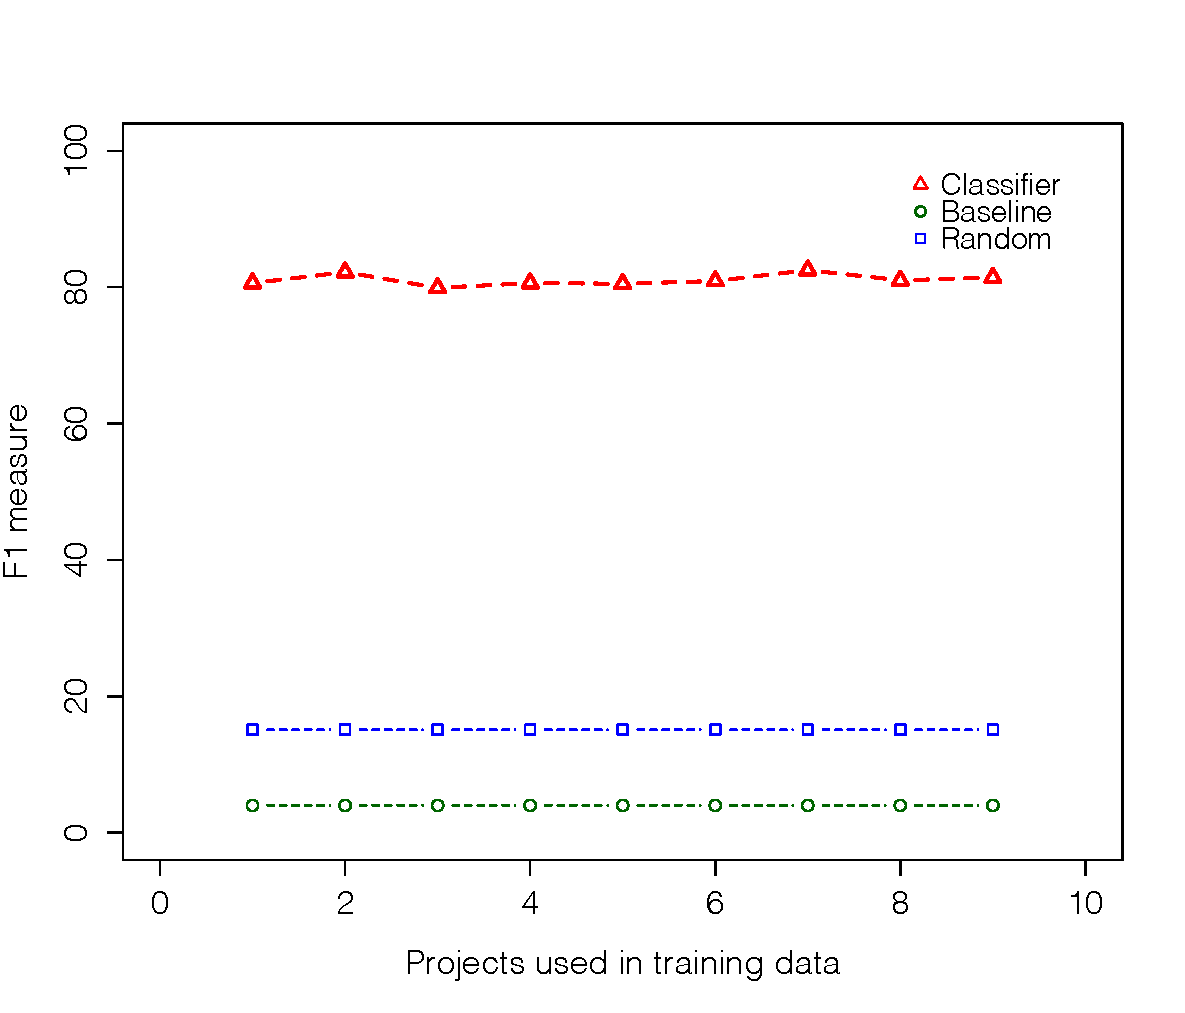
\includegraphics[width=0.50\textwidth]{figures/design_argo.pdf}
  \vspace{-3mm}
  \caption{Argo Design Debt classification}
  \label{fig:design_argo}
\end{figure}

\begin{figure}[thb!]
  \centering
  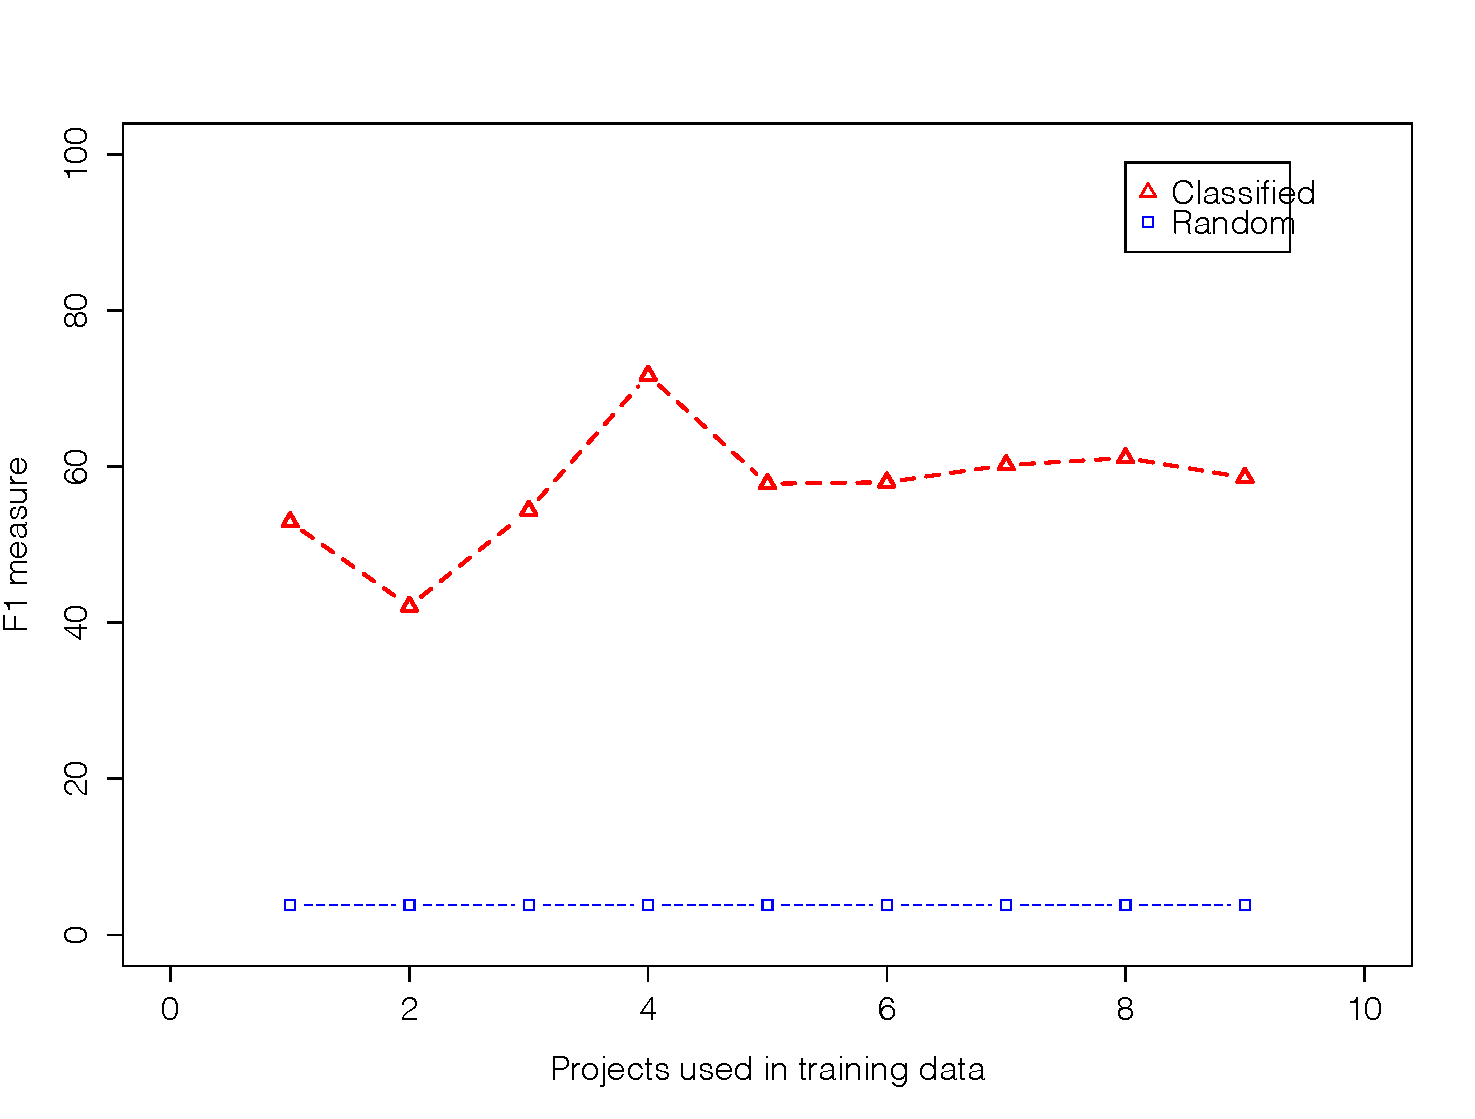
\includegraphics[width=0.50\textwidth]{figures/design_columba.pdf}
  \vspace{-3mm}
  \caption{Columba Design Debt classification}
  \label{fig:design_columba}
\end{figure}

\begin{figure}[thb!]
  \centering
  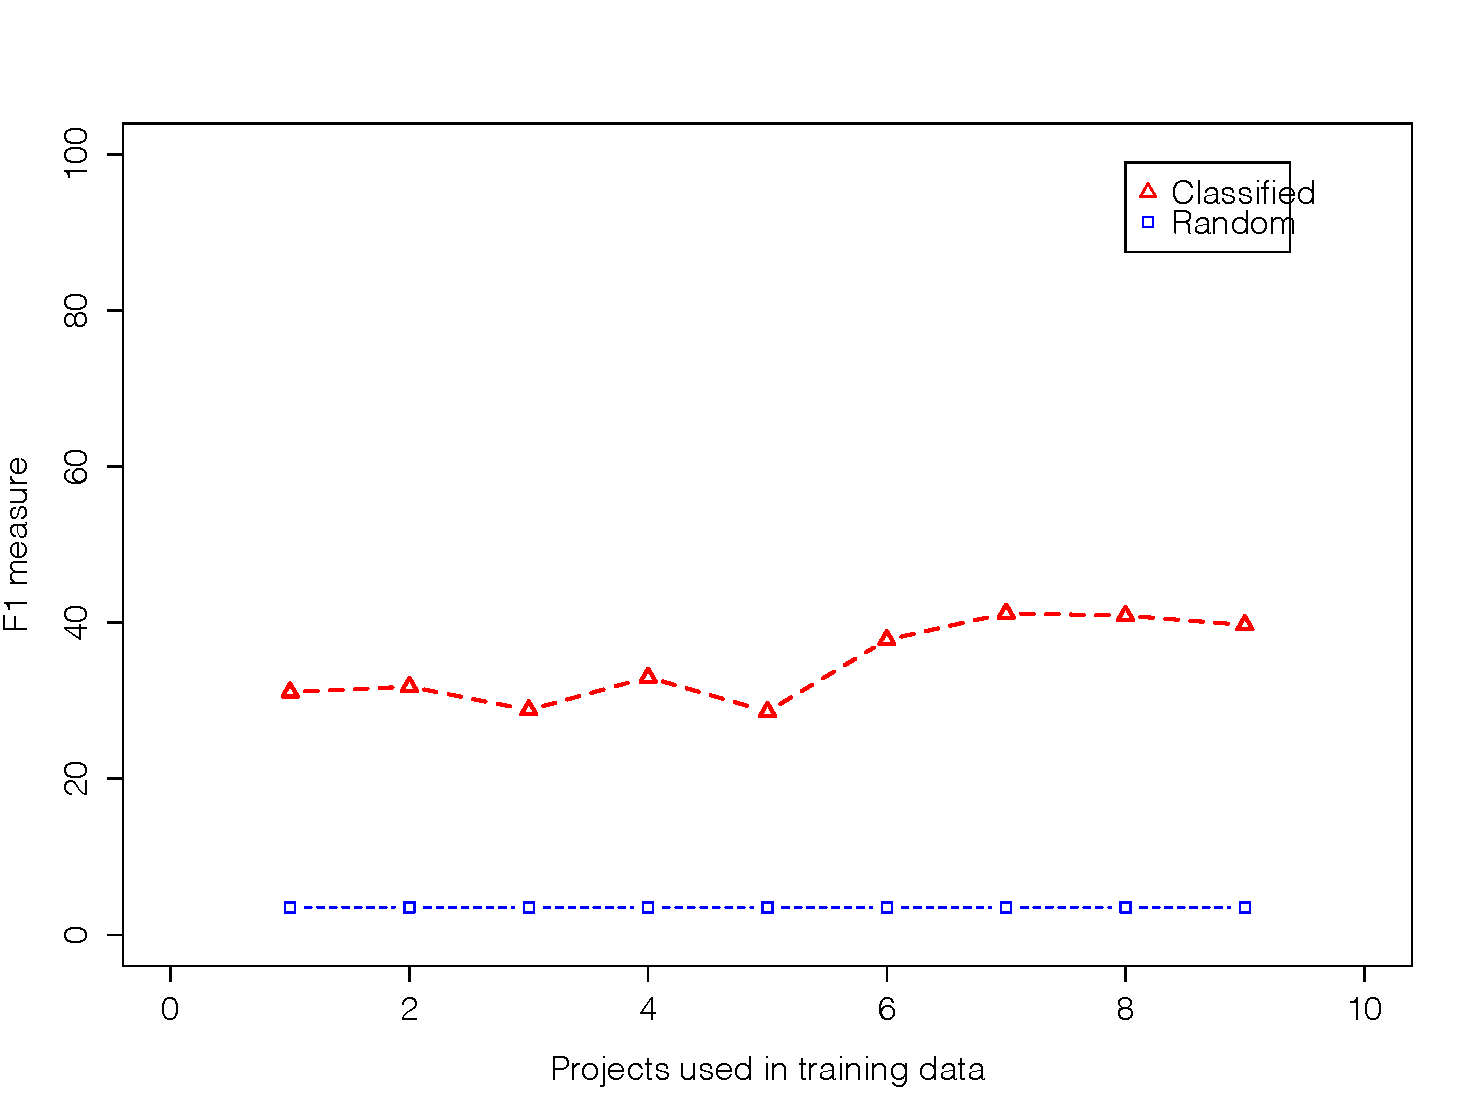
\includegraphics[width=0.50\textwidth]{figures/design_emf.pdf}
  \vspace{-3mm}
  \caption{Emf Design Debt classification}
  \label{fig:design_emf}
\end{figure}

\clearpage

\begin{figure}[thb!]
  \centering
  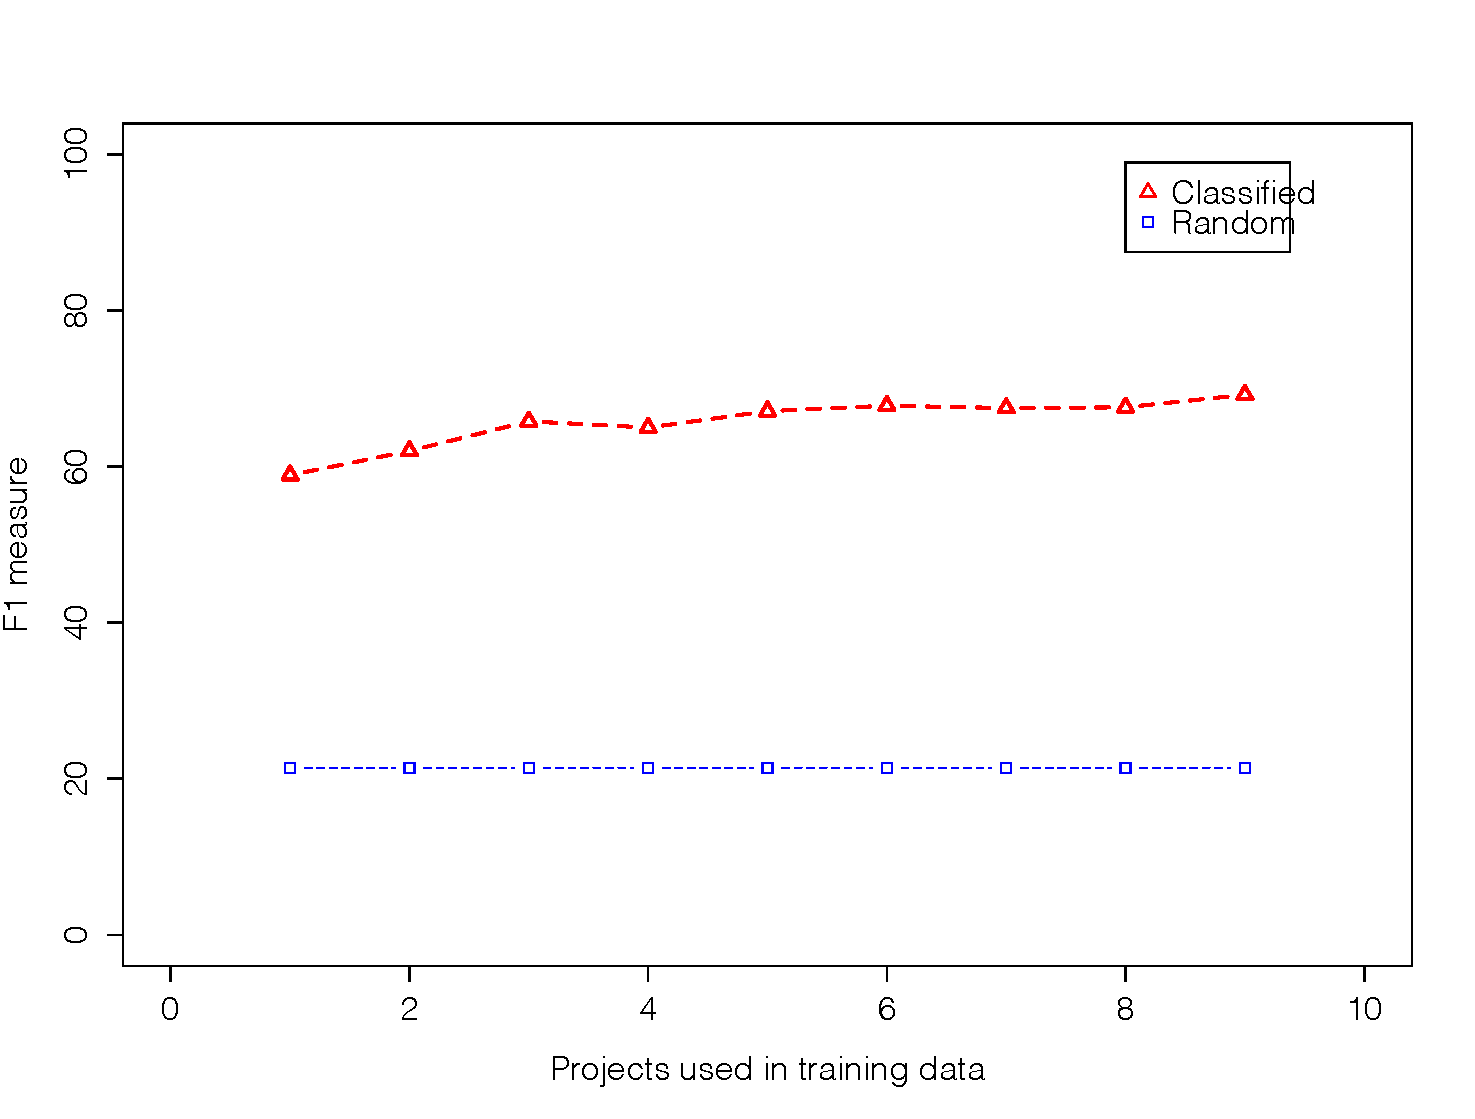
\includegraphics[width=0.50\textwidth]{figures/design_hibernate.pdf}
  \caption{Hibernate Design Debt classification}
  \label{fig:design_hibernate}
\end{figure}

\begin{figure}[thb!]
  \centering
  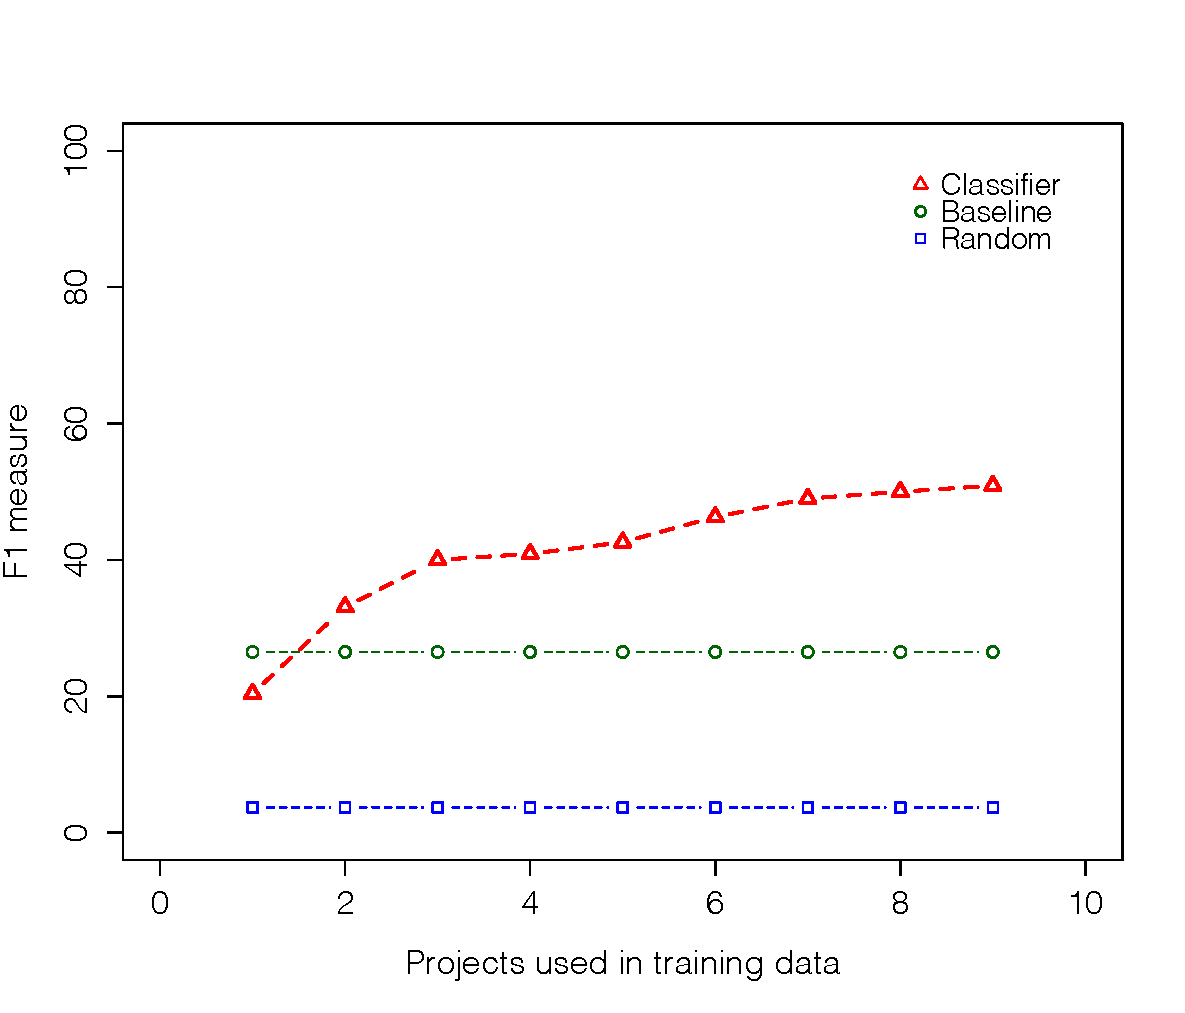
\includegraphics[width=0.50\textwidth]{figures/design_jedit.pdf}
  \vspace{-3mm}
  \caption{JEdit Design Debt classification}
  \label{fig:design_jedit}
\end{figure}

\begin{figure}[thb!]
  \centering
  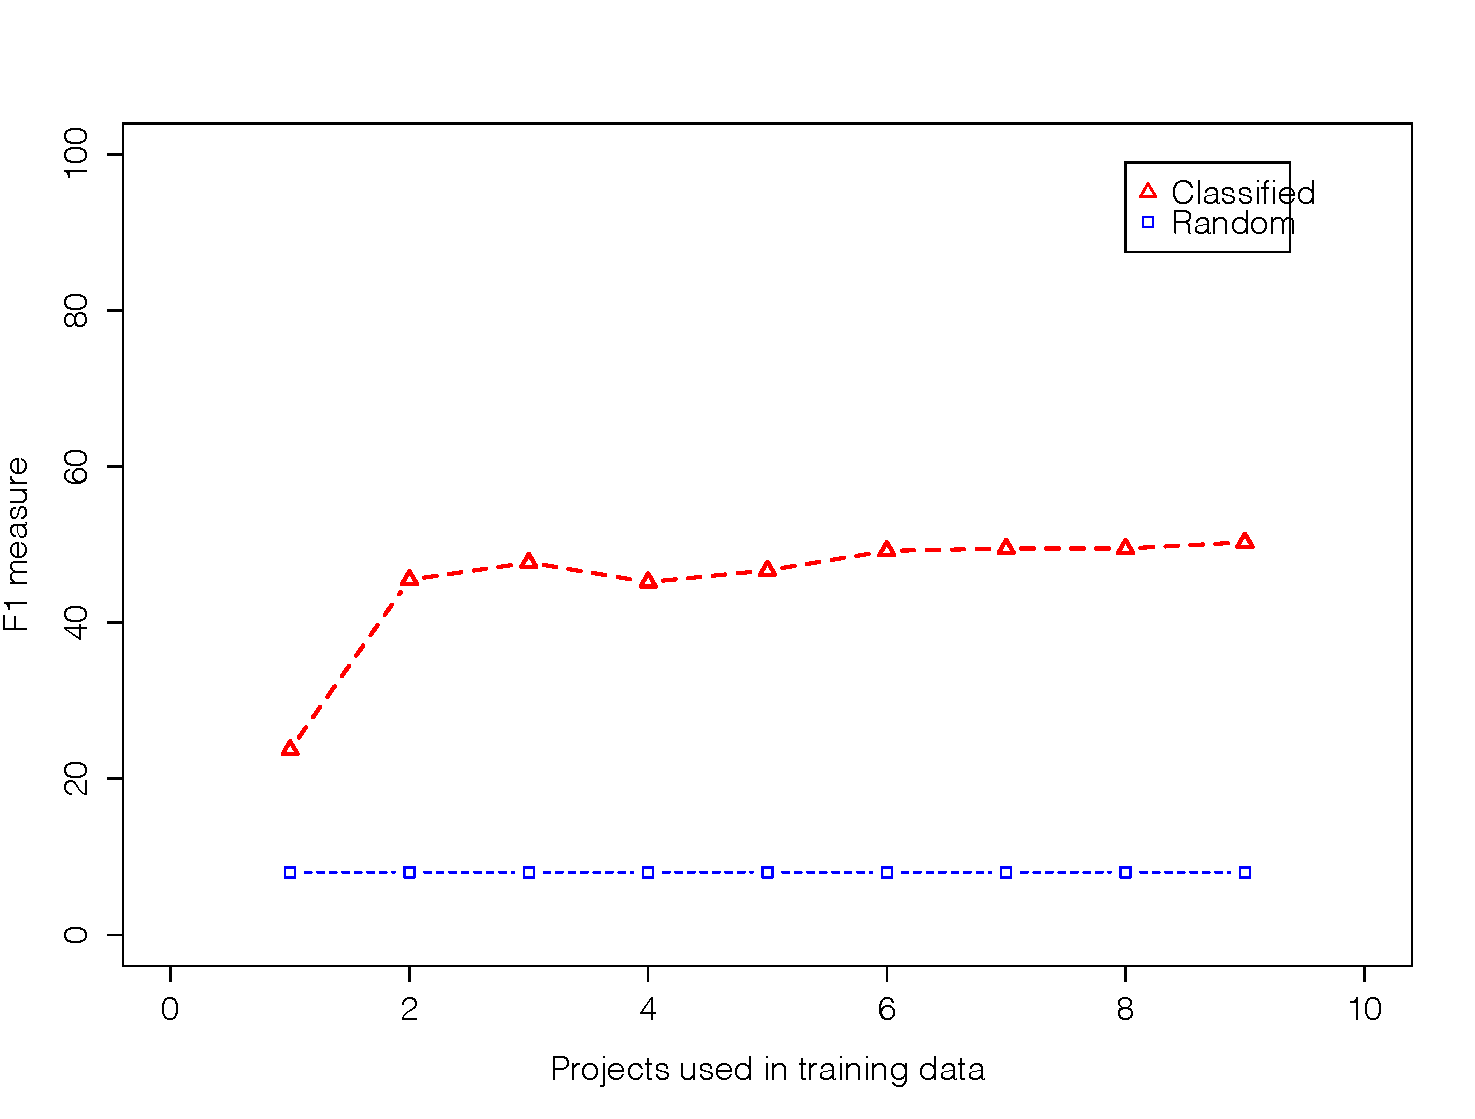
\includegraphics[width=0.50\textwidth]{figures/design_jfreechart.pdf}
  \vspace{-3mm}
  \caption{JFreeChart Design Debt classification}
  \label{fig:design_jfreechart}
\end{figure}

\begin{figure}[thb!]
  \centering
  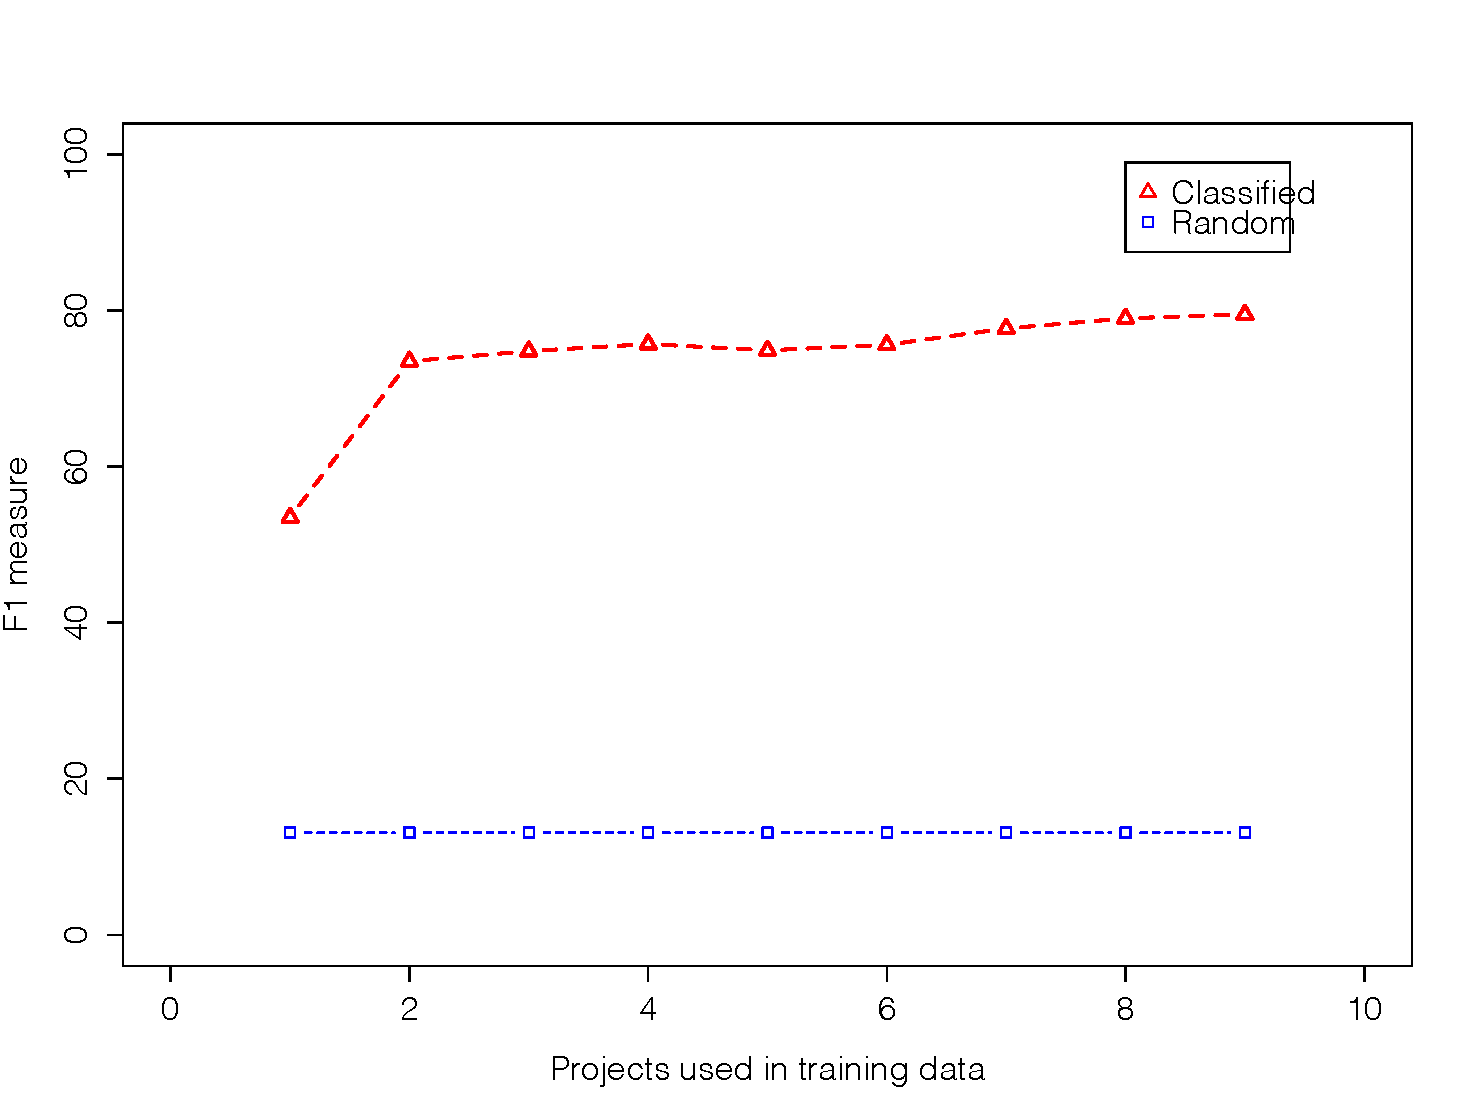
\includegraphics[width=0.50\textwidth]{figures/design_jruby.pdf}
  \vspace{-3mm}
  \caption{JRuby Design Debt classification}
  \label{fig:design_jruby}
\end{figure}

\begin{figure}[thb!]
  \centering
  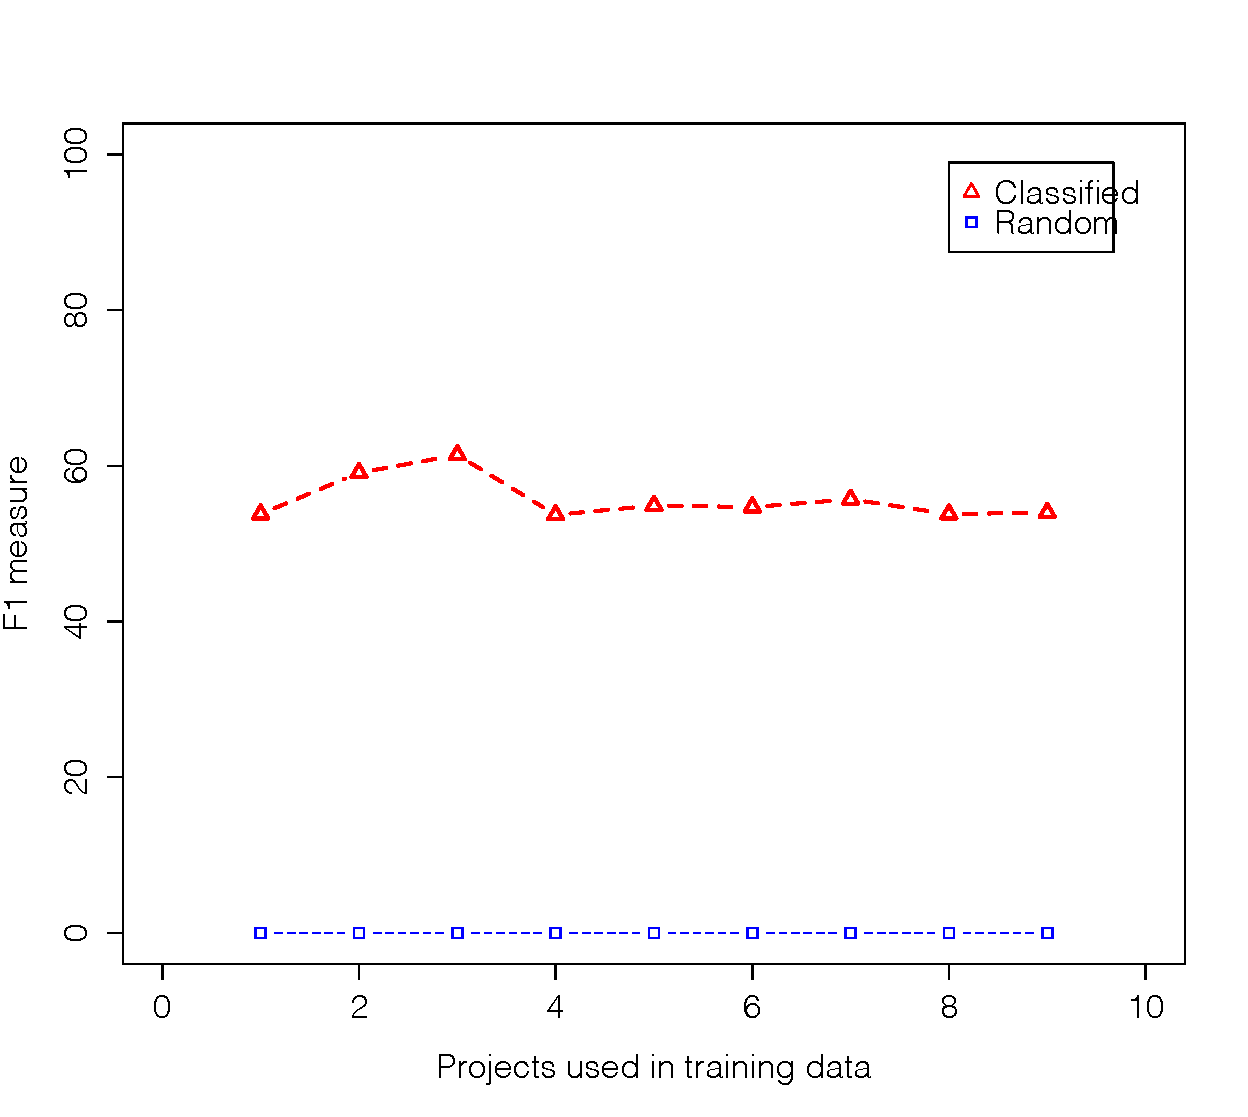
\includegraphics[width=0.50\textwidth]{figures/design_sql.pdf}
  \vspace{-3mm}
  \caption{SQuirrel Design Debt classification}
  \label{fig:design_sql}
\end{figure}

\clearpage
 
\begin{figure}[thb!]
  \centering
  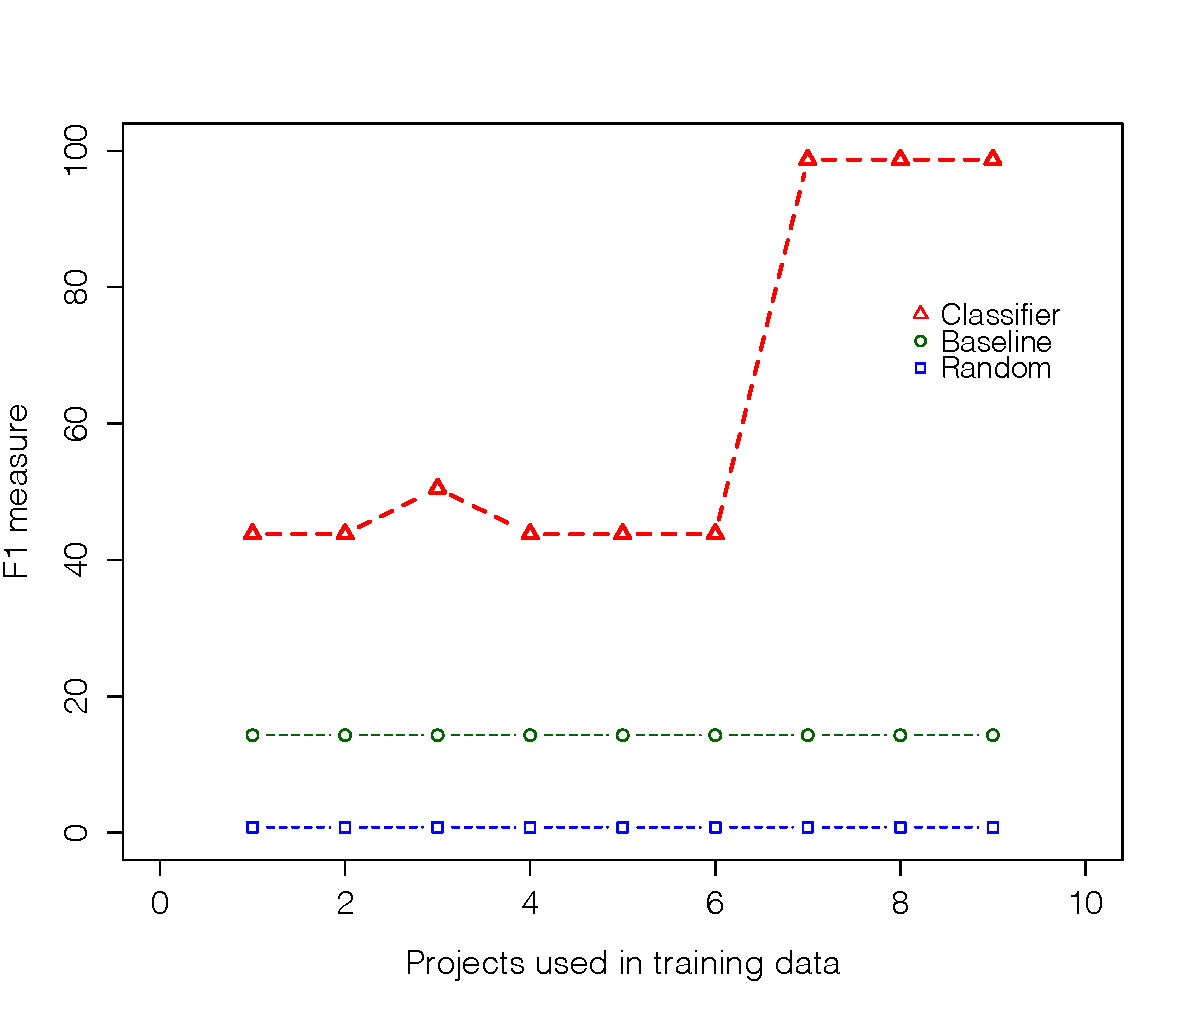
\includegraphics[width=0.50\textwidth]{figures/implementation_ant.pdf}
  \vspace{-3mm}
  \caption{Ant Requirement Debt classification}
  \label{fig:implementation_ant}
\end{figure}

\begin{figure}[thb!]
  \centering
  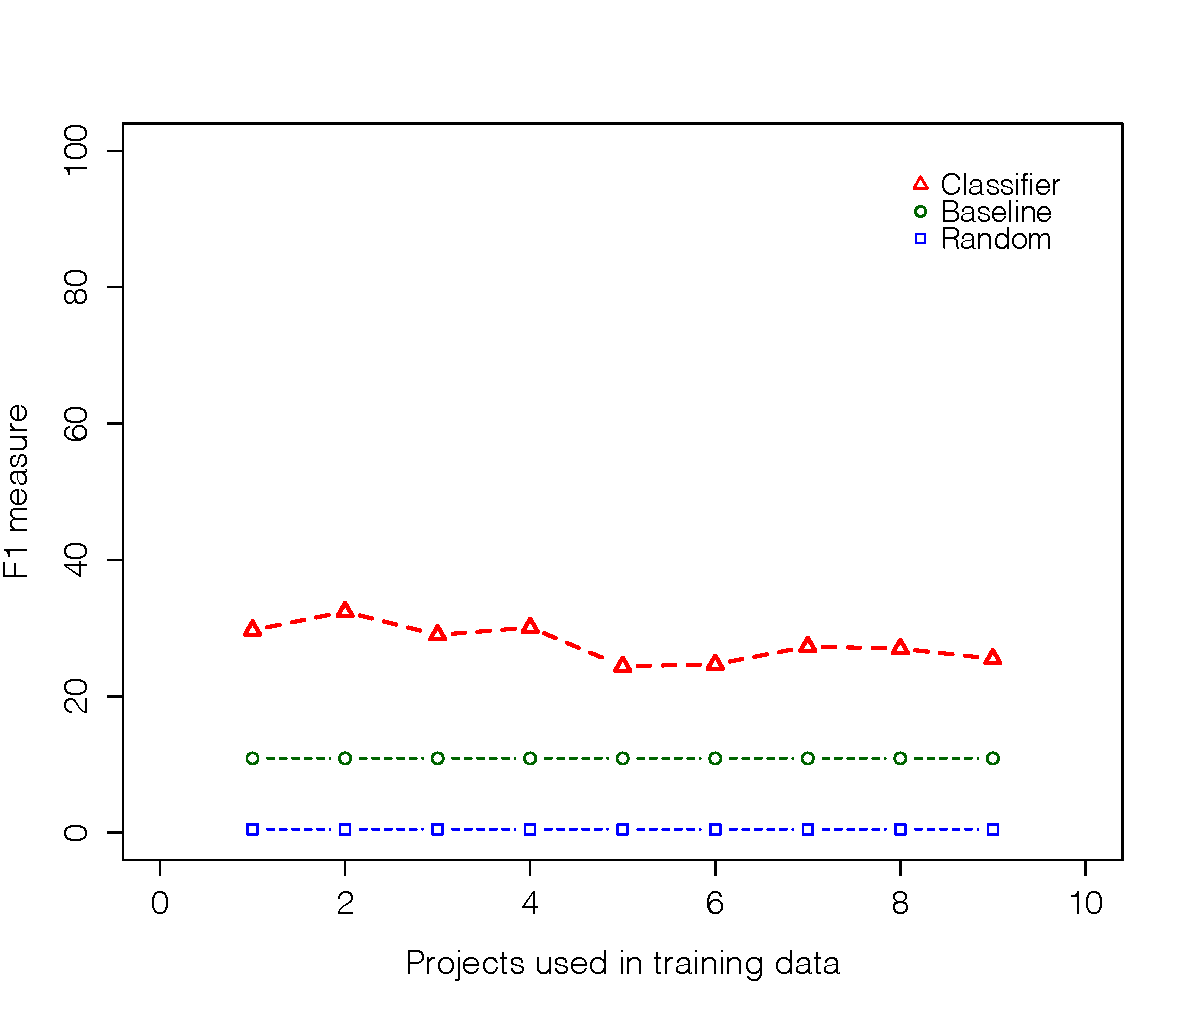
\includegraphics[width=0.50\textwidth]{figures/implementation_jmeter.pdf}
  \vspace{-3mm}
  \caption{Jmeter Requirement Debt classification}
  \label{fig:implementation_jmeter}
\end{figure}

\begin{figure}[thb!]
  \centering
  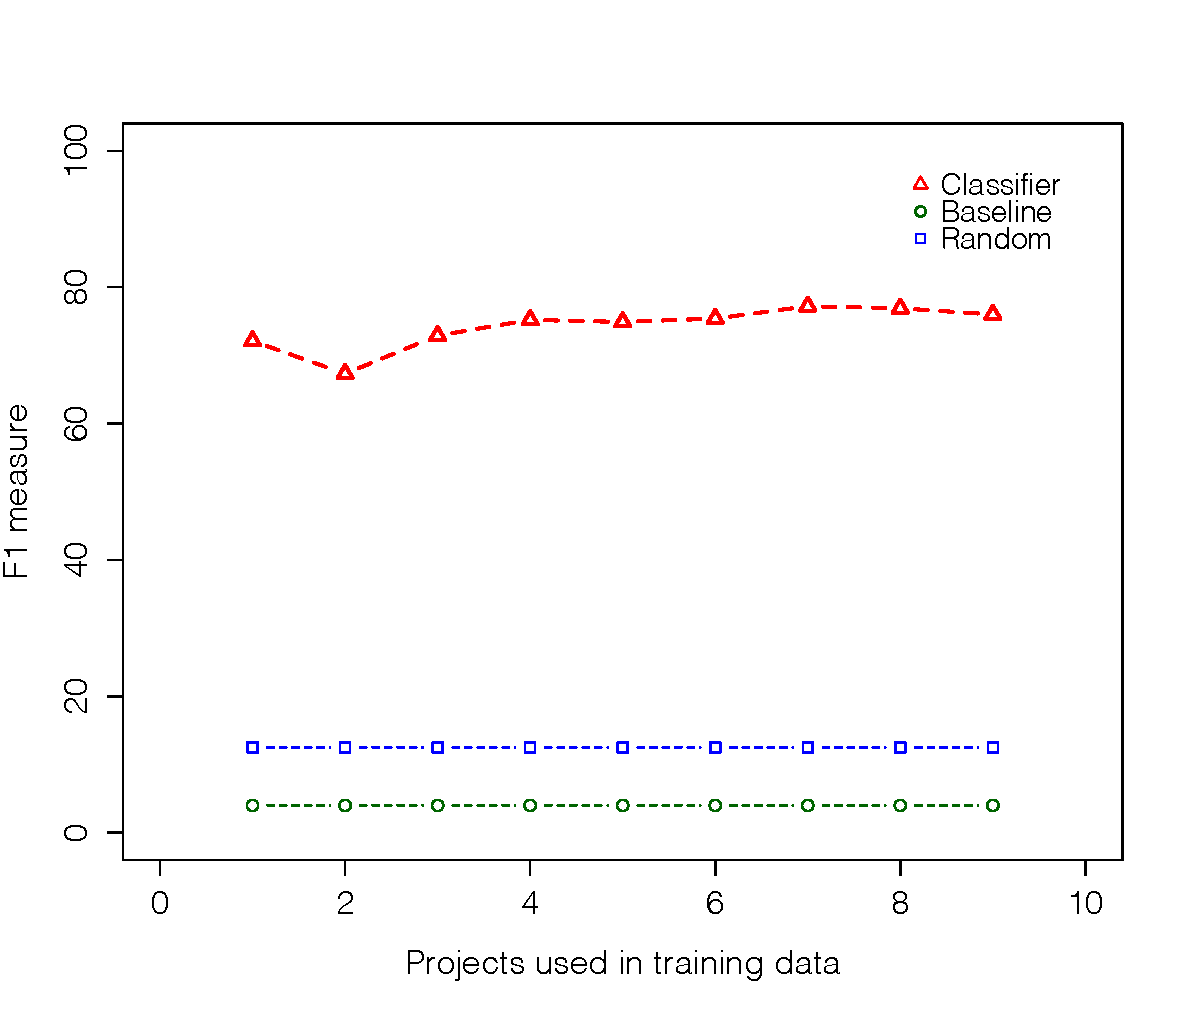
\includegraphics[width=0.50\textwidth]{figures/implementation_argo.pdf}
  \vspace{-3mm}
  \caption{Argo Requirement Debt classification}
  \label{fig:implementation_argo}
\end{figure}

\begin{figure}[thb!]
  \centering
  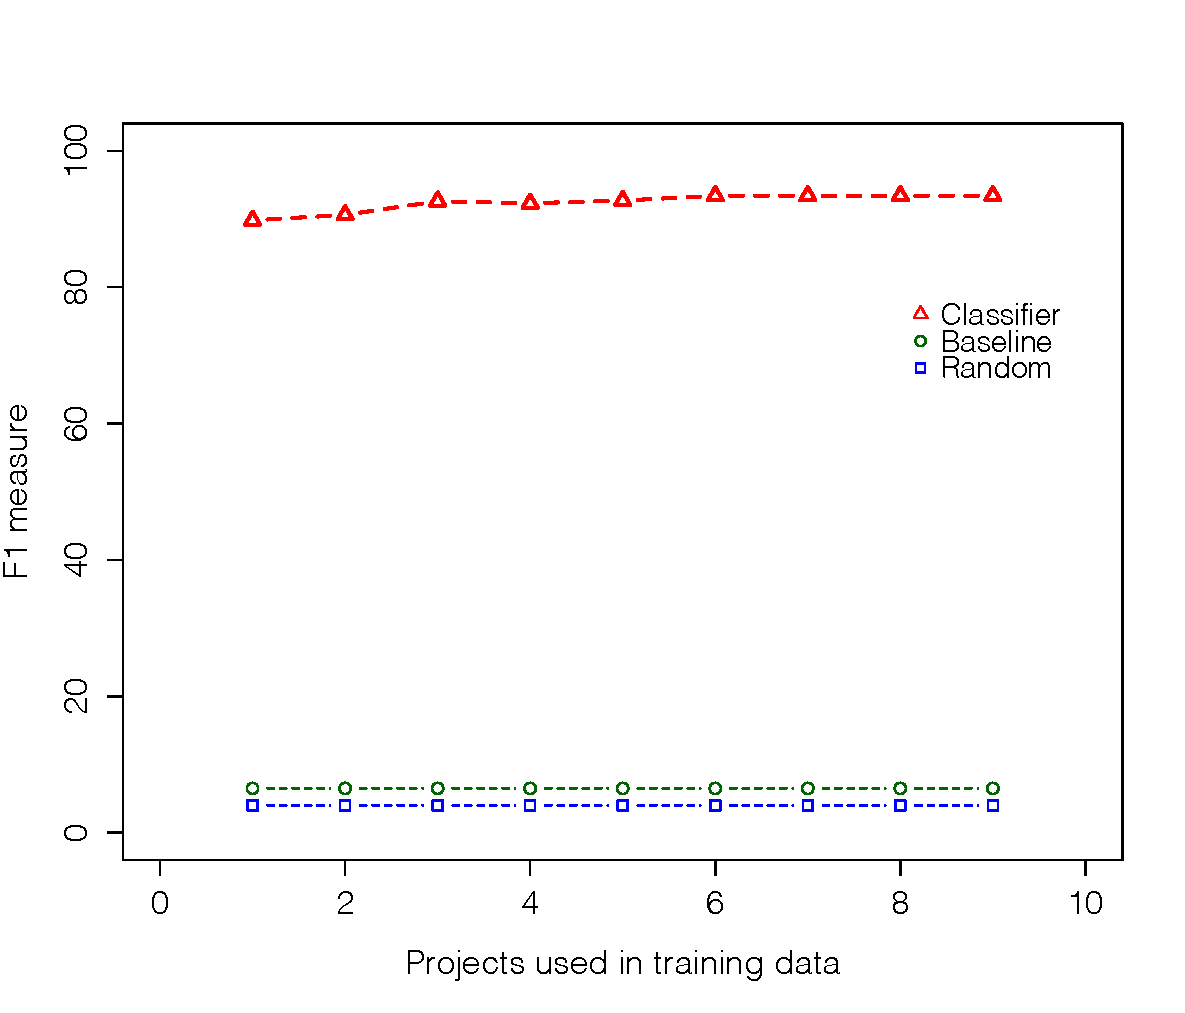
\includegraphics[width=0.50\textwidth]{figures/implementation_columba.pdf}
  \vspace{-3mm}
  \caption{Columba Requirement Debt classification}
  \label{fig:implementation_columba}
\end{figure}

\begin{figure}[thb!]
  \centering
  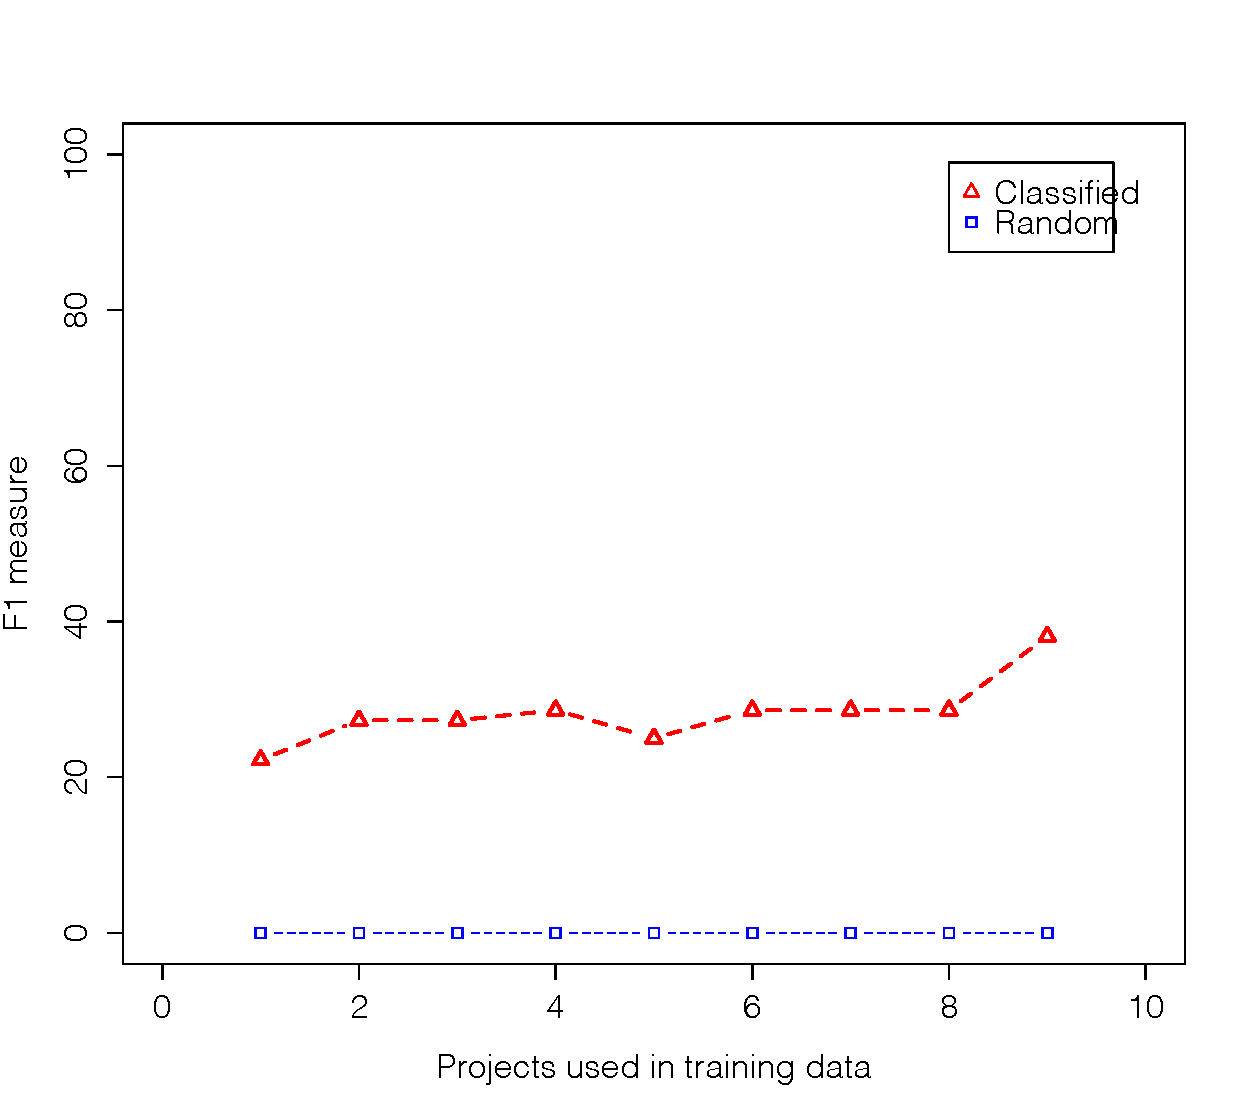
\includegraphics[width=0.50\textwidth]{figures/implementation_emf.pdf}
  \vspace{-3mm}
  \caption{Emf Requirement Debt classification}
  \label{fig:implementation_emf}
\end{figure}

\clearpage

\begin{figure}[thb!]
  \centering
  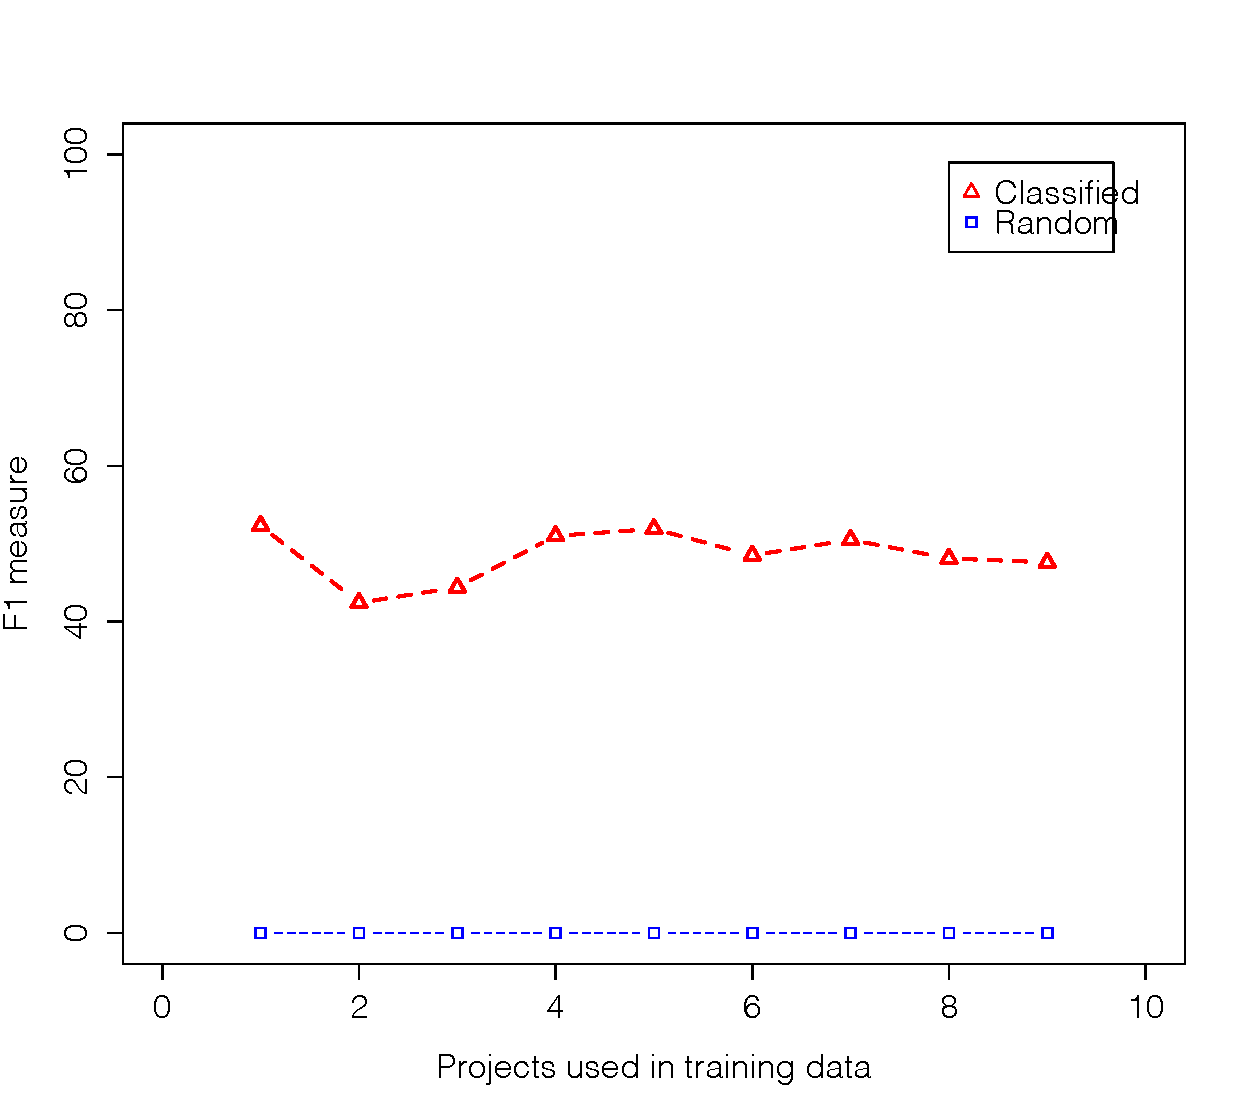
\includegraphics[width=0.50\textwidth]{figures/implementation_hibernate.pdf}
  \caption{Hibernate Requirement Debt classification}
  \label{fig:implementation_hibernate}
\end{figure}

\begin{figure}[thb!]
  \centering
  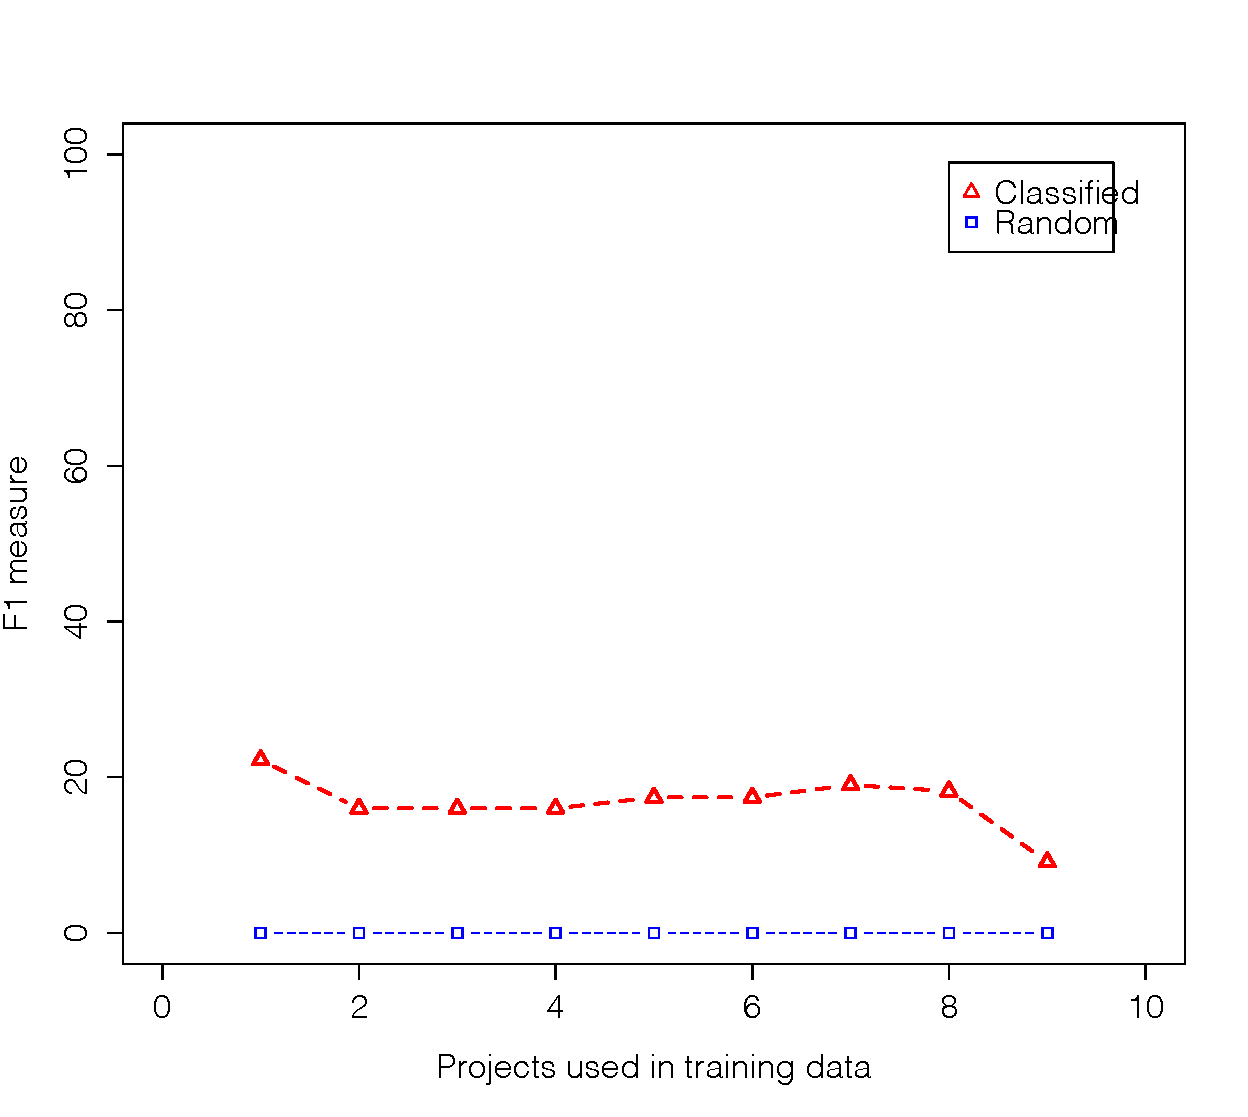
\includegraphics[width=0.50\textwidth]{figures/implementation_jedit.pdf}
  \vspace{-3mm}
  \caption{JEdit Requirement Debt classification}
  \label{fig:implementation_jedit}
\end{figure}

\begin{figure}[thb!]
  \centering
  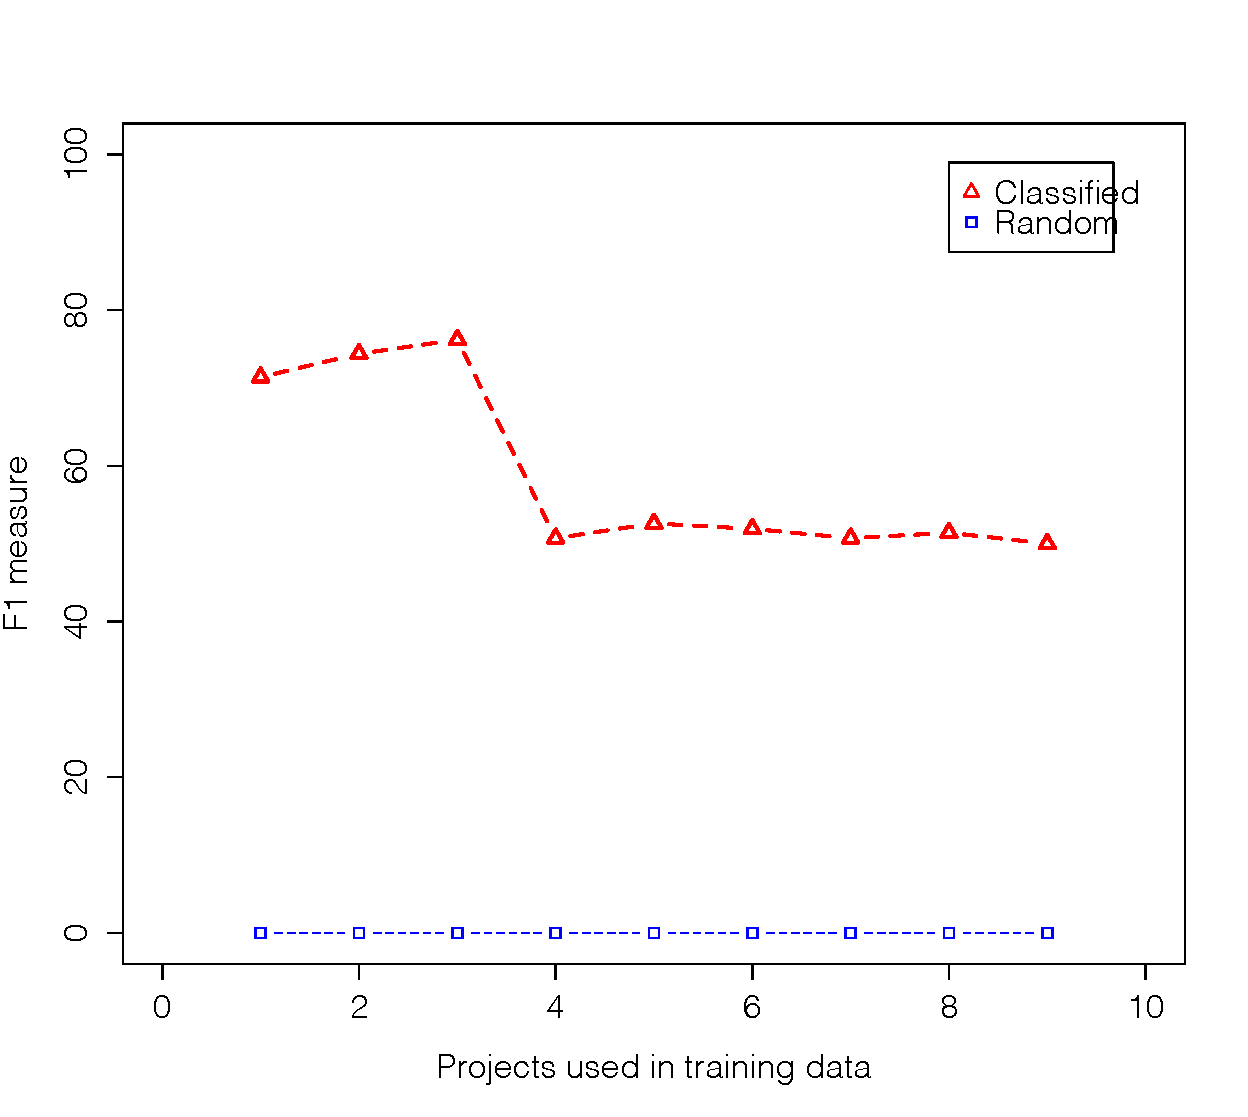
\includegraphics[width=0.50\textwidth]{figures/implementation_jfreechart.pdf}
  \vspace{-3mm}
  \caption{JFreeChart Requirement Debt classification}
  \label{fig:implementation_jfreechart}
\end{figure}

\begin{figure}[thb!]
  \centering
  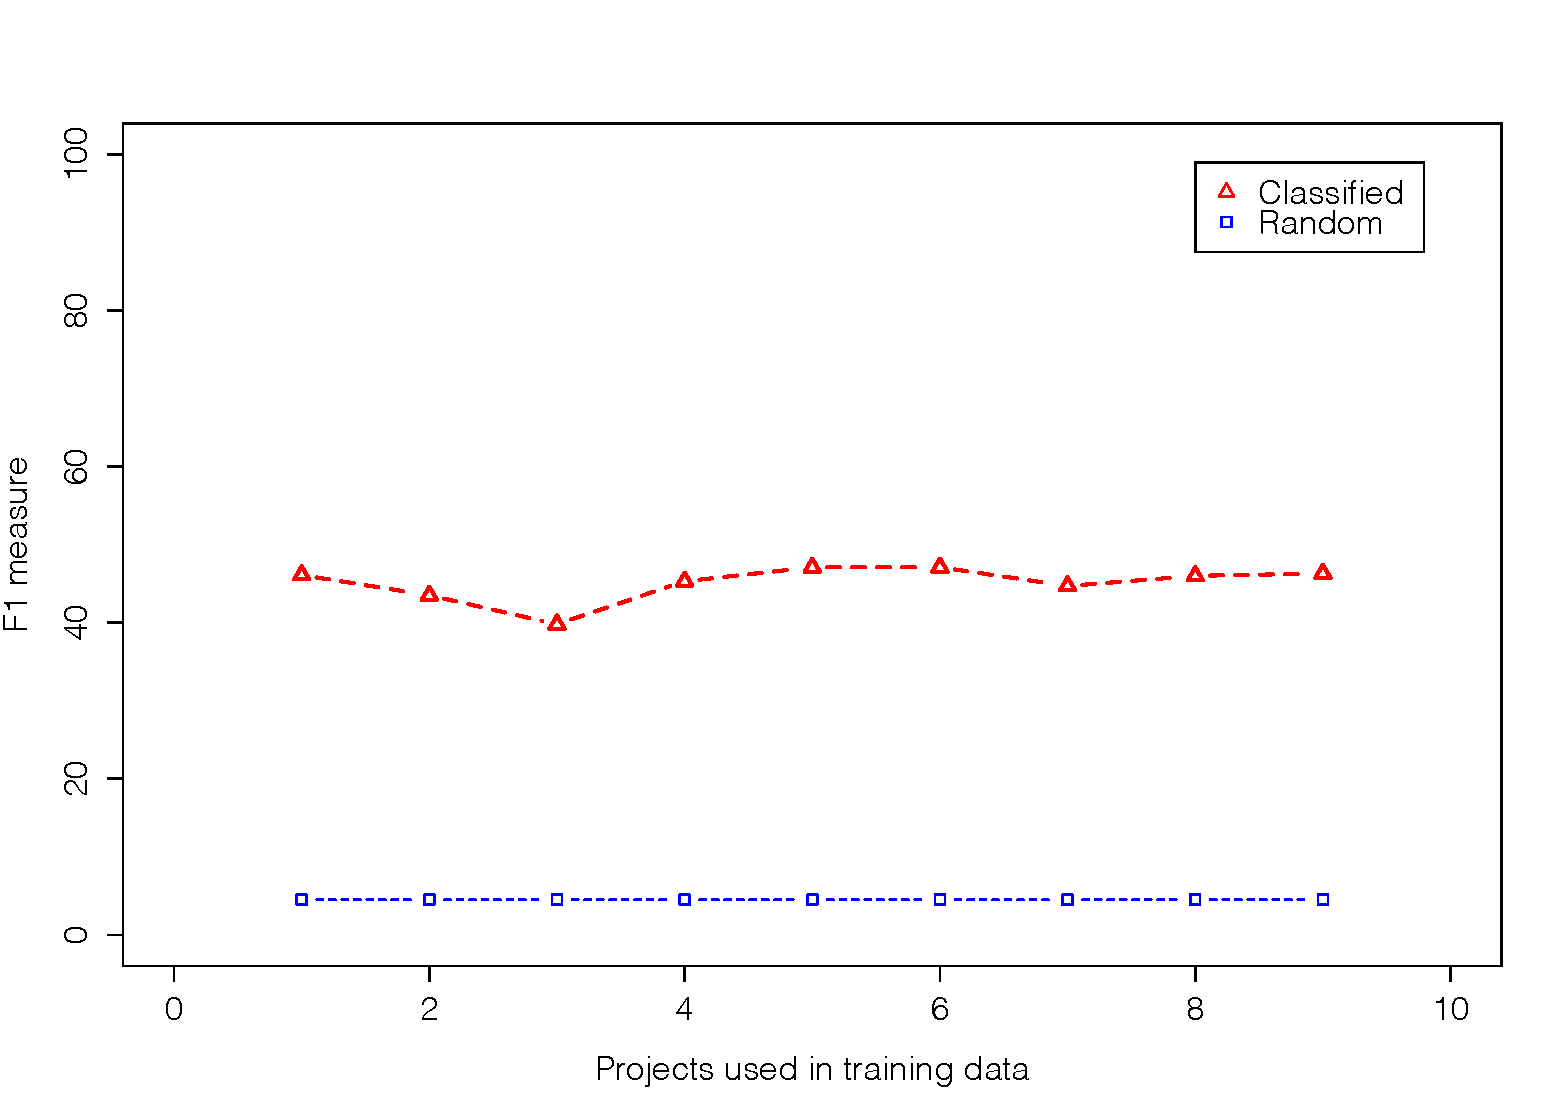
\includegraphics[width=0.50\textwidth]{figures/implementation_jruby.pdf}
  \vspace{-3mm}
  \caption{JRuby Requirement Debt classification}
  \label{fig:implementation_jruby}
\end{figure}

\begin{figure}[thb!]
  \centering
  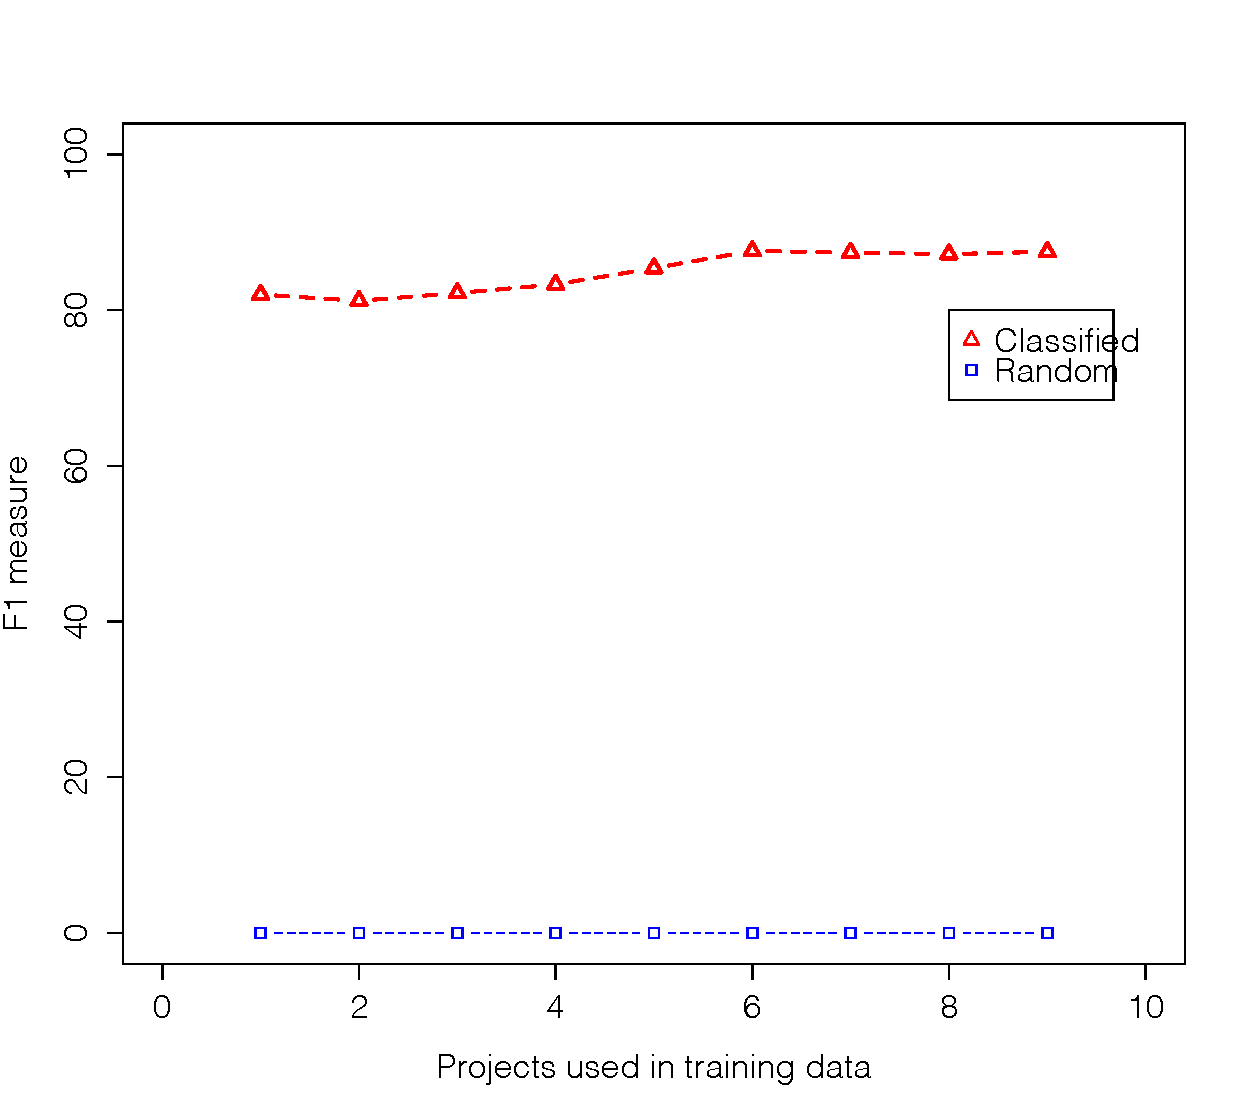
\includegraphics[width=0.50\textwidth]{figures/implementation_sql.pdf}
  \vspace{-3mm}
  \caption{SQuirrel Requirement Debt classification}
  \label{fig:implementation_sql}
\end{figure}

\clearpage

\begin{figure}[thb!]
  \centering
  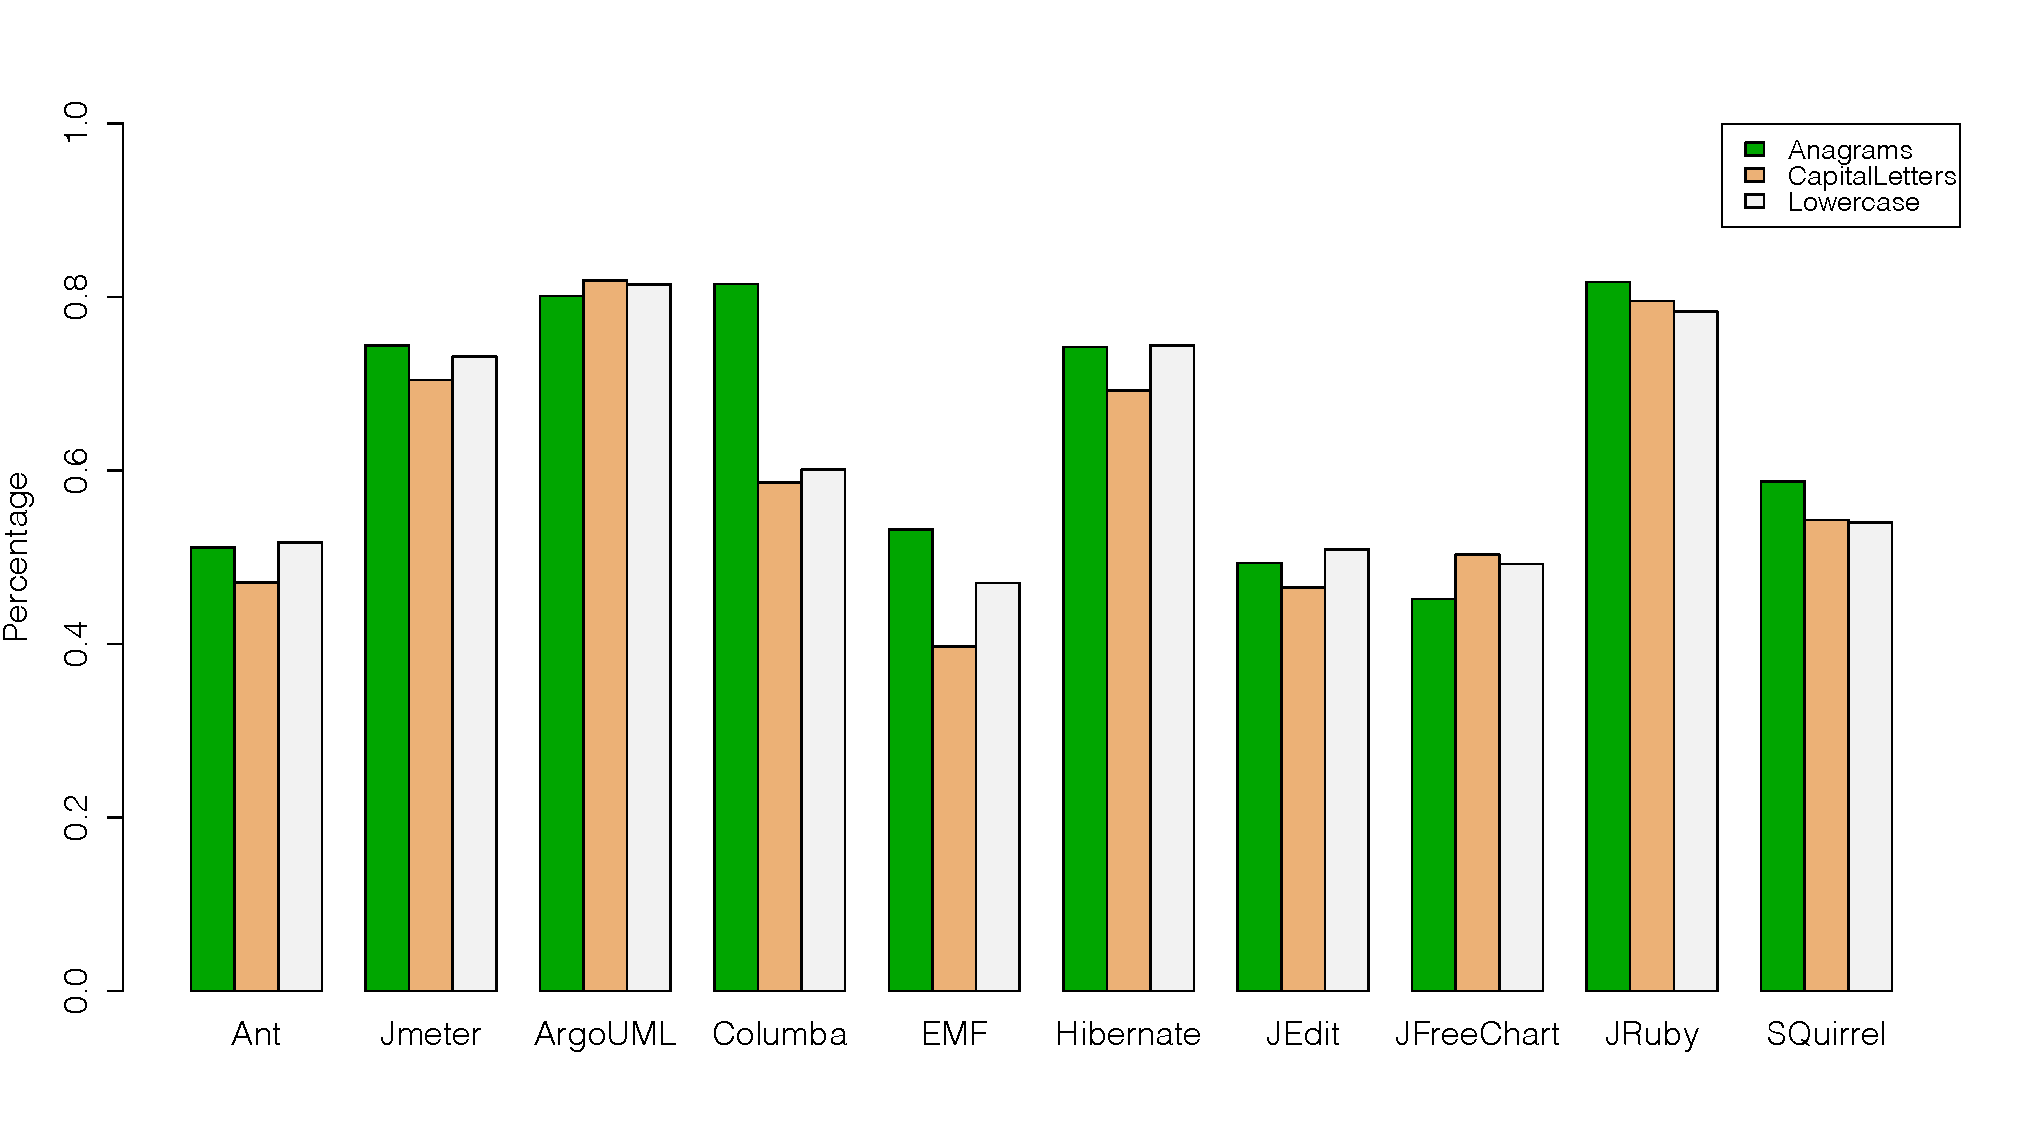
\includegraphics[width=0.50\textwidth]{figures/detailed_comparison_design_training_dataset.pdf}
  \vspace{-3mm}
  \caption{Detailed comparison of the changes in the design training datasets}
  \label{fig:detailed_comparison_design_training_dataset}
\end{figure}

\begin{figure}[thb!]
  \centering
  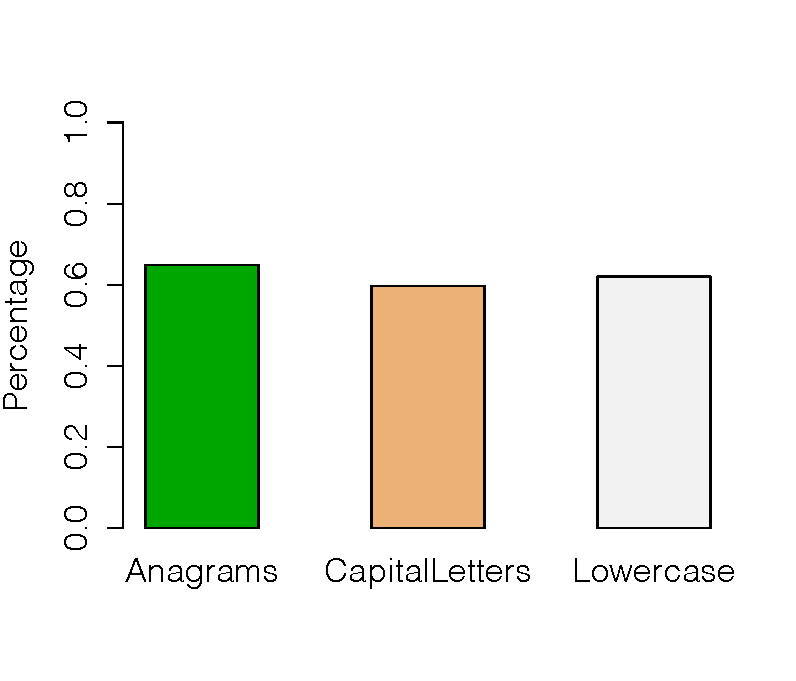
\includegraphics[width=0.50\textwidth]{figures/average_comparison_design_training_dataset.pdf}
  \vspace{-3mm}
  \caption{Average comparison of the changes in the design training datasets}
  \label{fig:average_comparison_design_training_dataset}
\end{figure}

\begin{table}[!hbt]
    \begin{center}
        \caption{Effects in the F1 measure of the Design training datasets}
        \label{tbl:detailed_comparison_design_training_dataset}
        \begin{tabular}{l| c c c}
        \toprule
        \thead{Project} & \thead{Anagrams\\Dataset} & \thead{Capitalized\\Dataset} & \thead{Lowercase\\Dataset}\\
        \midrule
        Apache Ant    &  0.511   & 0.471 &  0.517    \\
        Apache Jmeter &  0.744   & 0.704 &  0.731    \\
        ArgoUML       &  0.801   & 0.819 &  0.814    \\
        Columba       &  0.815   & 0.586 &  0.601    \\
        EMF           &  0.532   & 0.397 &  0.470    \\
        Hibernate     &  0.742   & 0.692 &  0.744    \\
        JEdit         &  0.493   & 0.465 &  0.509    \\
        JFreeChart    &  0.452   & 0.503 &  0.492    \\
        JRuby         &  0.817   & 0.795 &  0.783    \\
        SQuirrel      &  0.587   & 0.543 &  0.540    \\
        \bottomrule
        \end{tabular}
    \end{center}    
\end{table}

\clearpage

\begin{figure}[thb!]
  \centering
  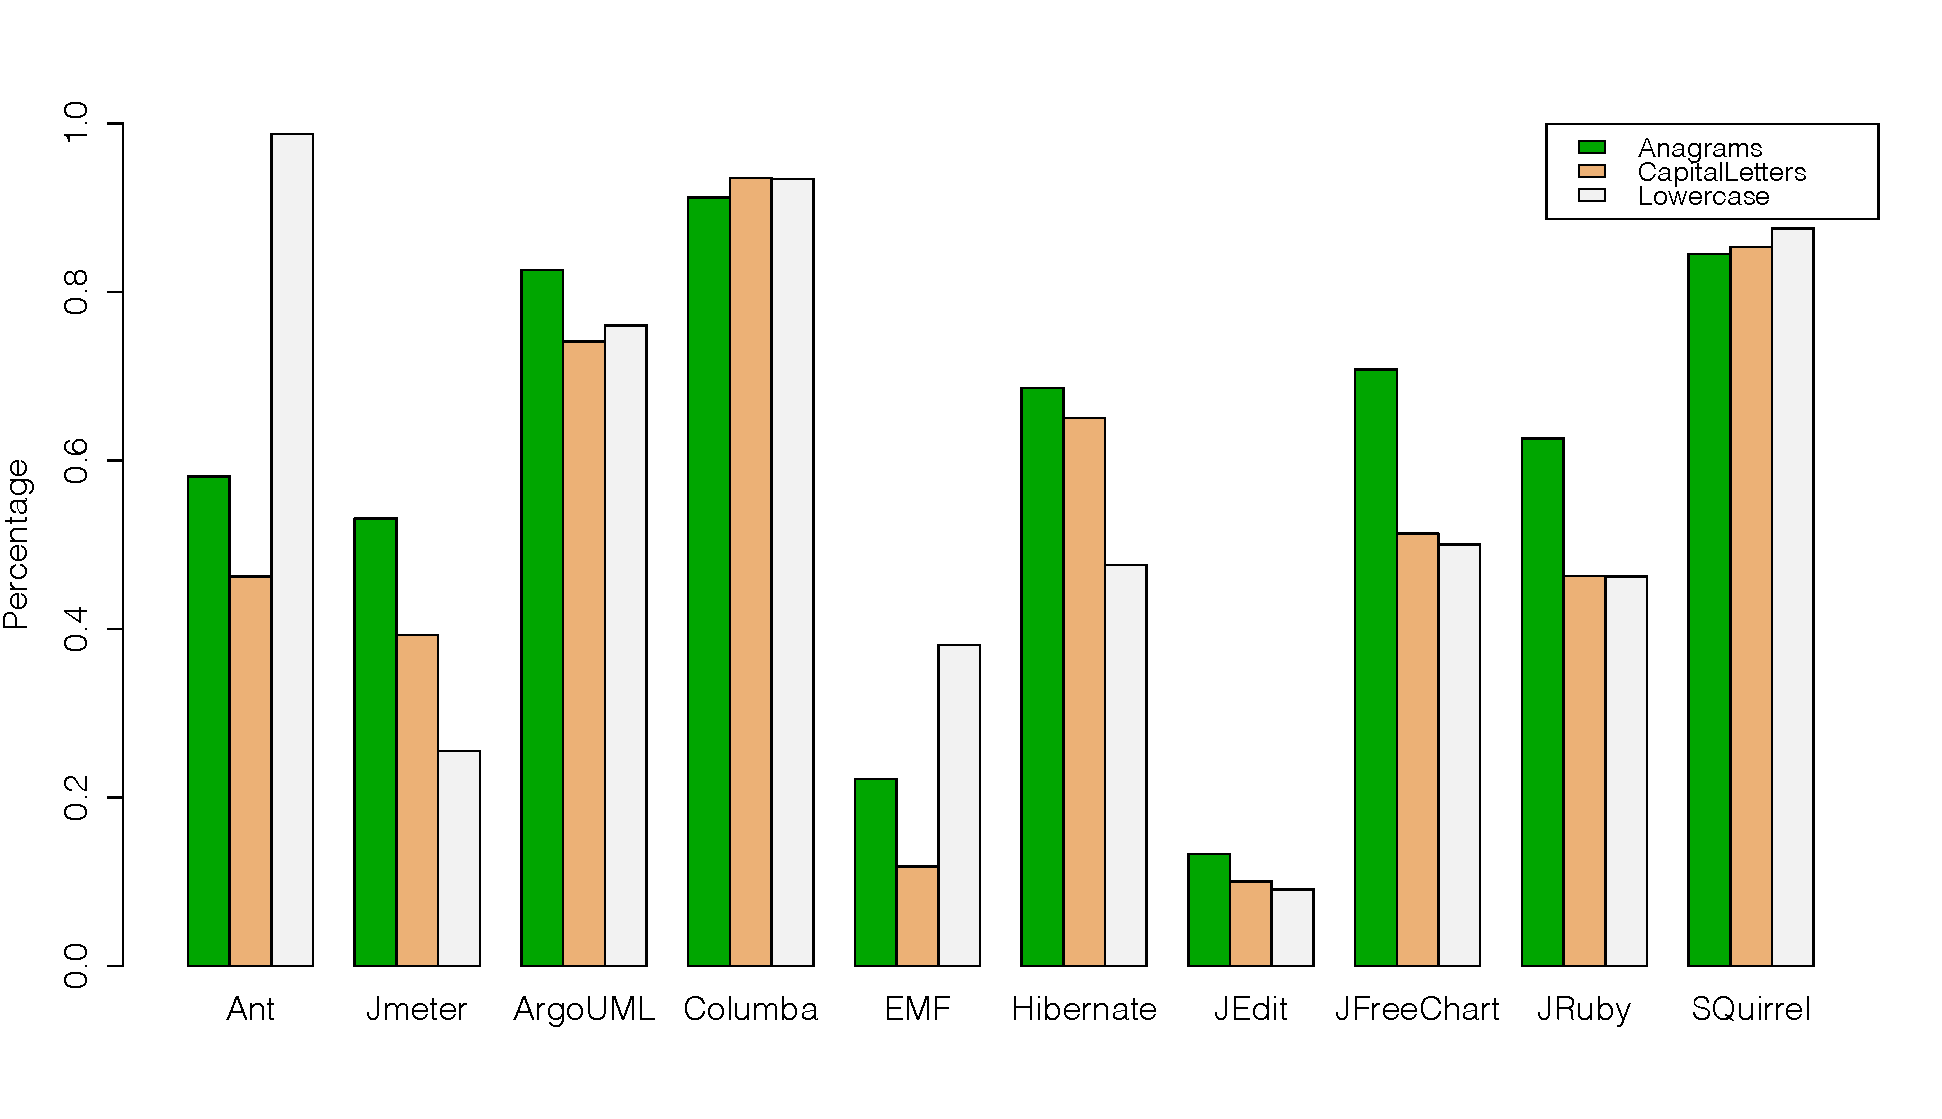
\includegraphics[width=0.50\textwidth]{figures/detailed_comparison_requirement_training_dataset.pdf}
  \vspace{-3mm}
  \caption{Detailed comparison of the changes in the requirements training datasets}
  \label{fig:detailed_comparison_requirement_training_dataset}
\end{figure}

\begin{figure}[thb!]
  \centering
  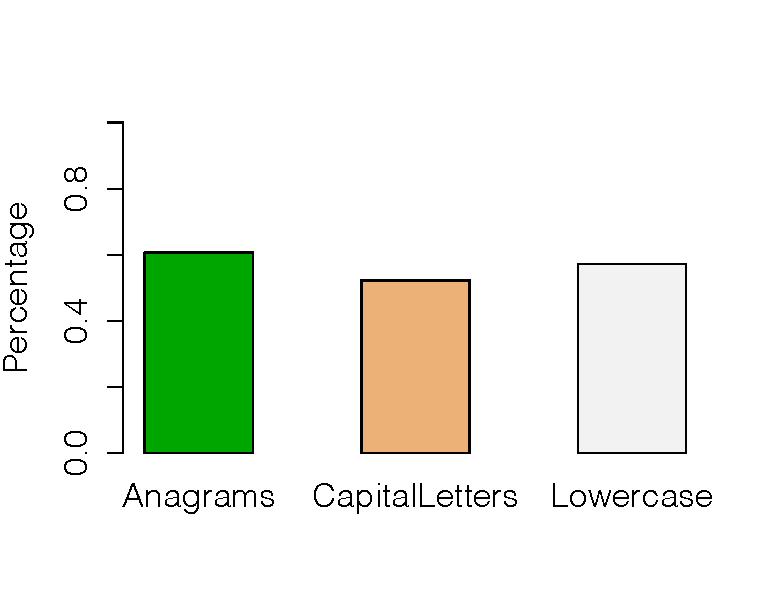
\includegraphics[width=0.50\textwidth]{figures/average_comparison_requeriment_training_dataset.pdf}
  \vspace{-3mm}
  \caption{Average comparison of the changes in the requirements training datasets}
  \label{fig:average_comparison_requirement_training_dataset}
\end{figure}

\begin{table}[!hbt]
    \begin{center}
        \caption{Effects in the F1 measure of the Requirements training datasets}
        \label{tbl:detailed_comparison_requirement_training_dataset}
        \begin{tabular}{l| c c c}
        \toprule
        \thead{Project} & \thead{Anagrams\\Dataset} & \thead{Capitalized\\Dataset} & \thead{Lowercase\\Dataset}\\
        \midrule
        Apache Ant    &  0.581 & 0.462 & 0.987  \\
        Apache Jmeter &  0.531 & 0.393 & 0.255  \\
        ArgoUML       &  0.826 & 0.741 & 0.760  \\
        Columba       &  0.912 & 0.935 & 0.934  \\
        EMF           &  0.222 & 0.118 & 0.381  \\
        Hibernate     &  0.686 & 0.650 & 0.476  \\
        JEdit         &  0.133 & 0.100 & 0.091  \\
        JFreeChart    &  0.708 & 0.513 & 0.500  \\
        JRuby         &  0.626 & 0.463 & 0.462  \\
        SQuirrel      &  0.845 & 0.853 & 0.875  \\
        \bottomrule
        \end{tabular}
    \end{center}    
\end{table}

